\documentclass[a4paper]{report}
\usepackage[utf8]{inputenc}
\usepackage[T1]{fontenc}   
\usepackage{m2rinfo}   
\usepackage[francais]{babel}  
\usepackage[top=3cm, bottom=2cm, left=3cm, right=3cm]{geometry}
\usepackage{setspace}
\usepackage[french,vlined,lined,boxed]{algorithm2e}
\usepackage{graphicx}
\usepackage{url}

\title{\huge{Application de tarot pour Android}}
\author{Bradshaw Kevin\\
Brunerie Sylvain\\
Buisson Roudet Jennifer\\
Hachiche Heykel\\ 
Subils Jean-Baptiste\\ 
Thill Fabrice}
\date{11 mai 2012}
\director{Mathieu  Lafourcade}
\laboratory{Université Montpellier 2}

\begin{document}
\maketitle


\tableofcontents





\chapter{Introduction}
	\section{Contexte pédagogique}
		Lors de notre troisième année en licence informatique à l’Université Montpellier 2, nous devons réaliser un projet pendant toute la durée du second semestre dans le cadre de l’Unité 			d’Enseignement GLIN601 : Projet Informatique. Ce module d’enseignement propose d’accomplir un projet technique en autonomie quasi complète et permet aux étudiants de développer 			plusieurs points importants tels que la notion de « projet » et la réutilisation des notions déjà acquises. Il s’inscrit dans la continuité des UE étudiées durant notre parcours 			(entre autres, GLIN505 Programmation par Objets et GLIN506 Conduite de Projet).\\
		\\ 

		Étant donné notre filière et notre enthousiasme pour les nouvelles technologies, nous avons proposé un sujet de développement sur une nouvelle plateforme pour appareils mobiles : Android. Il 			s’agit donc d’un projet purement pédagogique, qui nous permet de comprendre l’importance pour un informaticien de suivre l’actualité informatique ainsi que de se confronter 			régulièrement à de nouvelles technologies.\\
		\\ 
		Notre défi était donc d’effectuer un projet novateur, utile et agréable, et qui satisfasse les critères donnés pour le projet : quantité de travail, difficulté… Dès que le sujet fut 			validé par notre chef de filière, il nous a fallu trouver un enseignant volontaire pour encadrer ce projet. Ce projet s’est donc déroulé sous la tutelle de M. Mathieu Lafourcade, maître 			de conférences au LIRMM.\\
		\\  
		L’objet de ce projet consiste à développer une application de tarot sur la plateforme Android. Cela permettra à la fois de découvrir la programmation sous ce système d’exploitation open 			source dédié aux smartphones et d’en évaluer le potentiel, et les modalités de développement. Le but de ce projet était donc dans un premier temps de découvrir la plate-forme de Google, et les outils qui gravitent 			autour (émulateur, SDK…). Une fois familiarisé avec l’environnement, nous devions prendre en main les concepts du développement pour appareils mobiles et de manière plus précise 			comprendre le fonctionnement des applications destinés à Android.\\
	\section{Sujet}
		Ce projet de développement sous Android, encadré par M. Lafourcade, s’insère dans un projet de découverte de cette nouvelle plateforme pour téléphonie mobile ou encore tablettes.\\
  		L'objectif de ce TER est de créer un jeu de tarot qui vise la plateforme android, avec une intelligence artificielle.\\
    		Au début du projet, l’objectif de ce module consistait seulement à la création d'une interface graphique Android qui permettrait de jouer à un jeu à quatre joueurs, un contre trois intelligences 			artificielles.\\
  		Cependant des objectifs secondaires été proposés tels que la possibilité de jouer en ligne, à 3, 4 ou 5.


\chapter{Les règles du tarot}
		Le jeu de tarot est un jeu de cartes qui est apparu en Europe au cours du XVe siècle. Les cartes de tarots sont surtout connues pour leur utilisation dans des arts divinatoires.
	\section{À propos du jeu de tarot}
		Le tarot est un jeu de cartes. Il se joue généralement à quatre joueurs, il existe cependant des variantes très répandues pour pouvoir jouer avec trois et cinq joueurs.\\
		Il existe également d’autres variantes pour le jeu à deux, six joueurs ou plus, mais beaucoup moins connues.\\
		Le Tarot est un jeu plutôt vieux et comporte des règles qui varient selon l’habitude des joueurs.\\

	\section{Les cartes}
		Le jeu de tarot comporte 78 cartes, dont 56 cartes de couleur, 21 atouts, et l’Excuse.\\
		Comme dans la plupart des jeux de cartes, il y a quatre couleurs : coeur, pique, carreau et trèfle. Chaque couleur est constituée de 14 cartes. Dans l'ordre décroissant de force et de 		valeur : Roi, Dame, Cavalier et Valet, qui constituent les Honneurs (ou les Habillés, ou les Têtes) ; puis 10, 9, 8, 7, 6, 5, 4, 3, 2, 1.\\
		Les Atouts (ou Tarots) sont des cartes numérotées qui ont priorité sur les couleurs. Le numéro indique la force de chaque atout, du plus fort, le 21, au plus faible, le 1 appelé 			Le Petit.\\
		Enfin l'Excuse, une carte marquée d'une étoile et représentant un joueur de mandoline, est une sorte de « joker » jouable n’importe quand, et qui est toujours récupérée par le 		camp de celui qui l’a joué (sauf s’il l’a jouée au dernier tour, auquel cas elle revient au camp adverse).\\
	\section{La distribution}


		La distribution au Tarot est un peu particulière, elle suit des règles bien précises. Le donneur commence à distribuer au joueur situé après lui, suivant le sens prédéfini (sens 			inverse ou non des aiguilles d’une montre). Il doit distribuer les cartes trois par trois pour chaque joueur, et de temps en temps en mettre une ou plusieurs au « chien », un 			ensemble de trois (à 5 joueurs) ou six cartes (à 3 et 4 joueurs) qui n’appartient à ce moment à aucun des joueurs (son sort sera déterminé pendant la phase d’annonces). Le 			donneur ne peut pas mettre au chien la première ni la dernière carte du tas.\\
		\\ 
		L’ajout d’une carte se fait aléatoirement entre les distribution pour chaque joueur suivant les personnes l’ajout des cartes au chien se fait soit une par une soit on peut 			choisir de rajouter 1 à 3 cartes.\\
			La distribution au tarot est un peu particulière, elle suit des règles bien précises. Le donneur commence à distribuer au joueur situé après lui, suivant le sens prédéfini (sens 			inverse ou non des aiguilles d’une montre). Il doit distribuer les cartes trois par trois pour chaque joueur, et de temps en temps en mettre une ou plusieurs au « chien », un 			ensemble de trois (à 5 joueurs) ou six cartes (à 3 et 4 joueurs) qui n’appartient à ce moment à aucun des joueurs (son sort sera déterminé pendant la phase d’annonces). Le 			donneur ne peut pas mettre au chien la première ni la dernière carte du tas.\\
			\begin{center}
				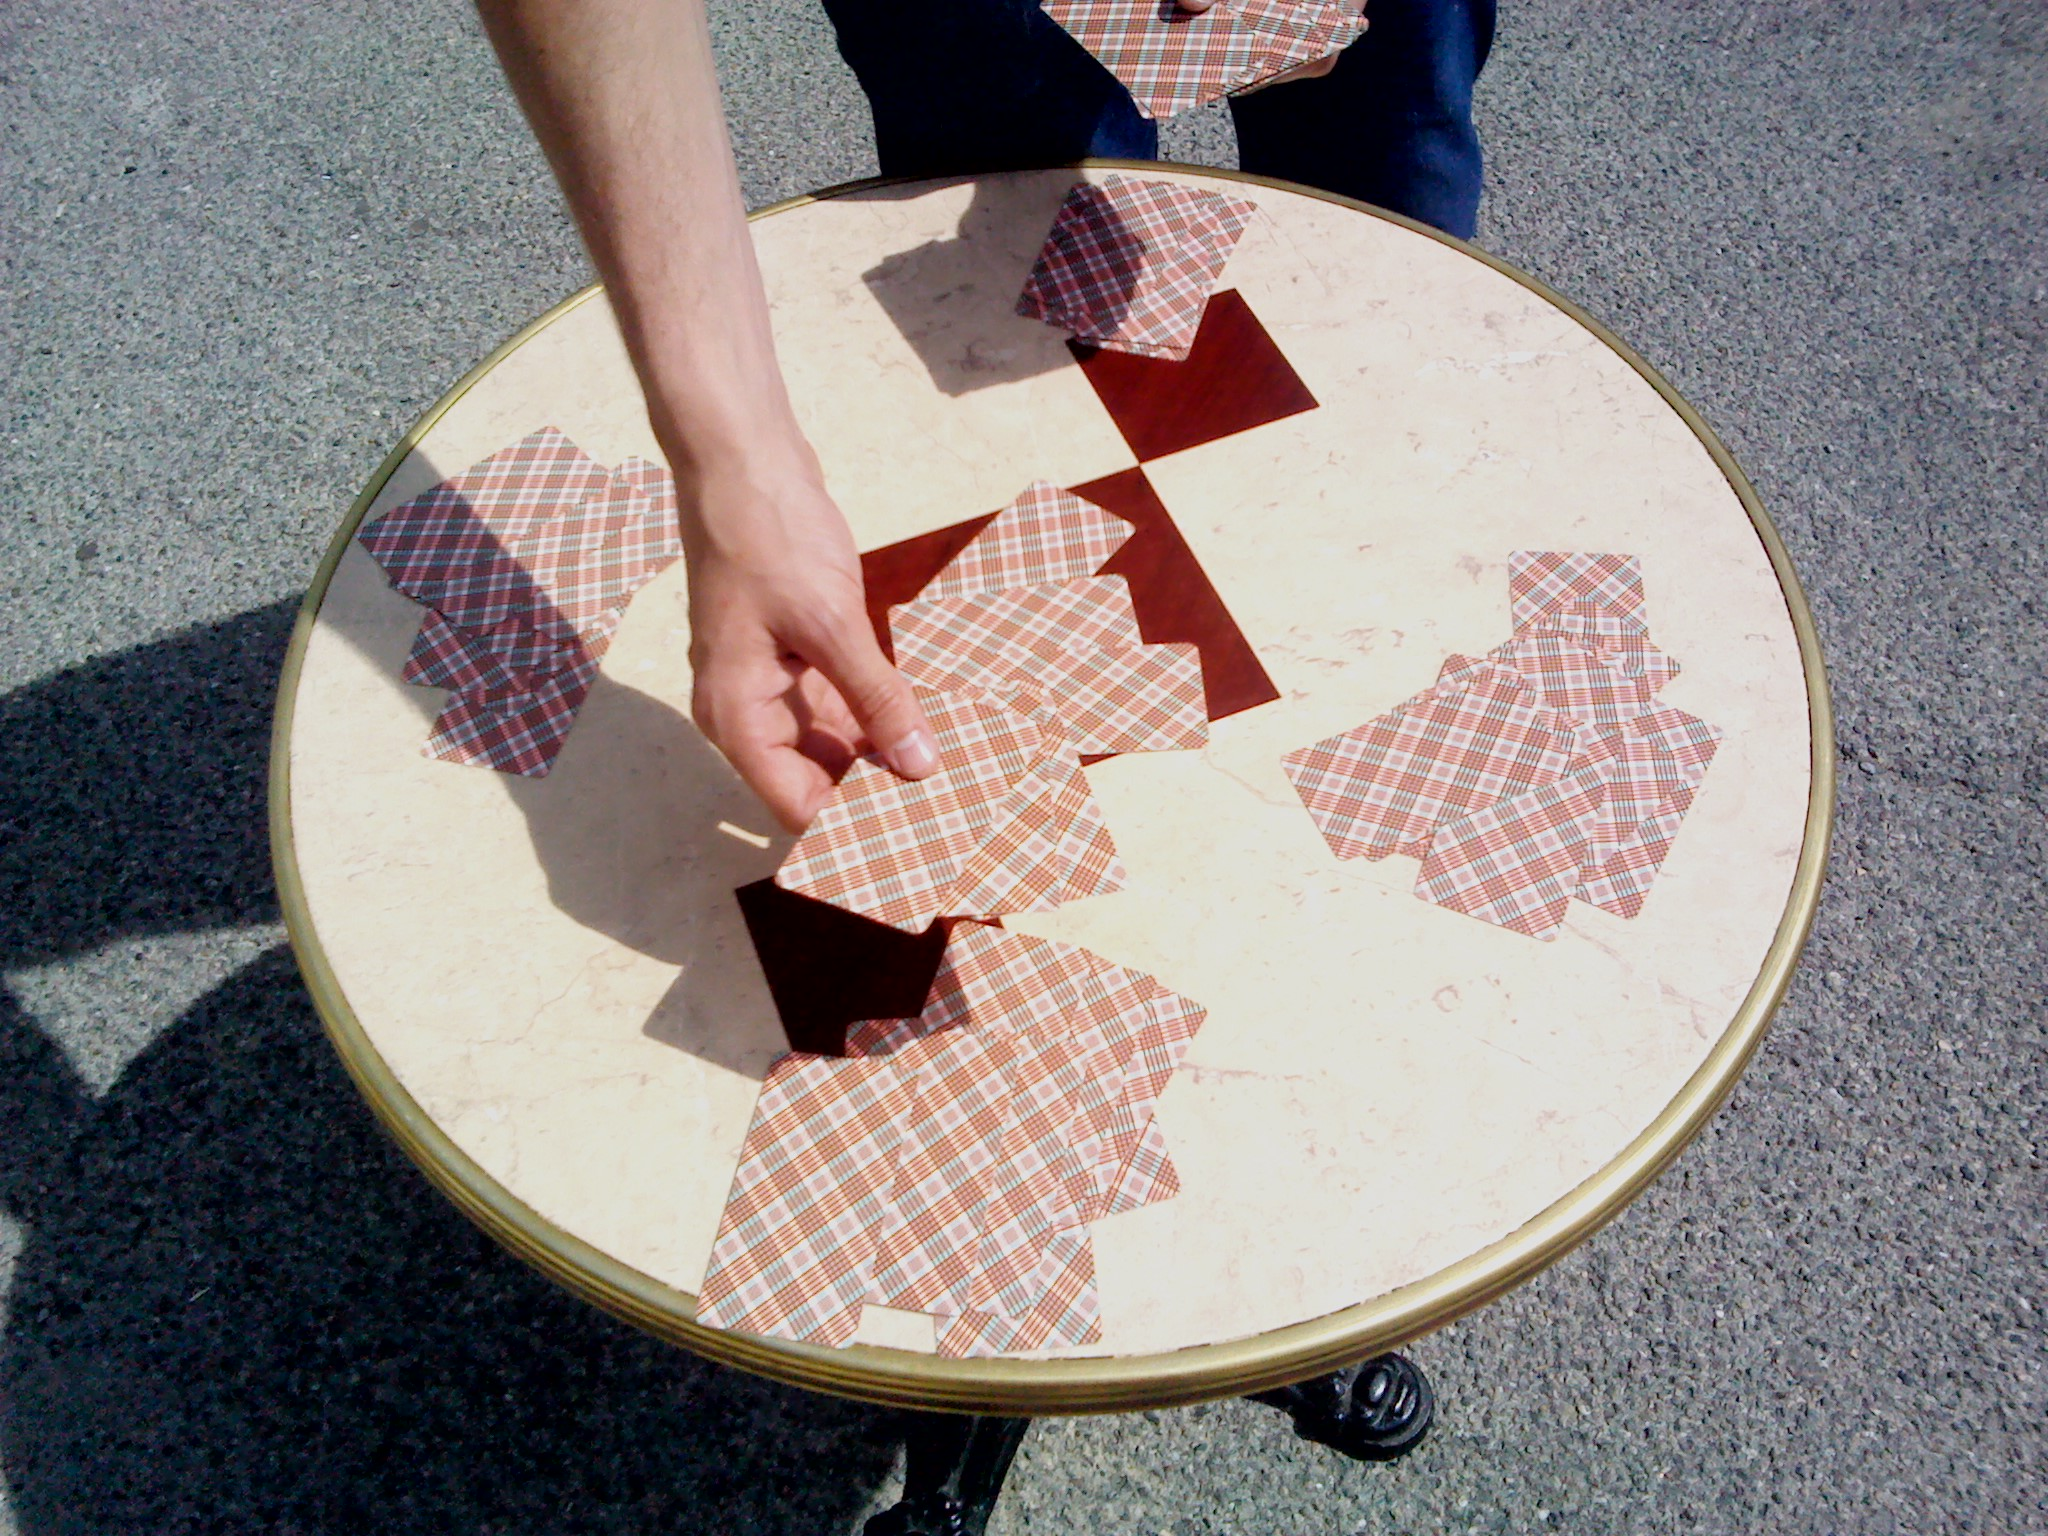
\includegraphics[scale=0.15]{Images/3.jpg}
			\end{center}
	\section{Les annonces / Les enchères}
		
		Dans la phase d’annonces, qui suit la distribution, le premier joueur à parler est celui situé après le donneur. Chaque joueur va annoncer à son tour, jusqu’à ce que les 			annonces soient terminées.\\
			Trois cas de figure sont possibles :
		\begin{itemize}
				\item Tout le monde a passé ;
  				\item L’annonce la plus haute (Garde contre) a été faite ;
   				\item Il ne reste plus qu’une personne à annoncer.
		\end{itemize}
			Une fois qu’un joueur a passé, il ne peut plus parler.\\
		\begin{itemize}
   				\item Passe : le joueur ne veut pas prendre.
   				\item Petite ou Prise : le joueur veut prendre mais avec peu de risques.
   				\item Garde : le joueur veut prendre mais il met plus de points en jeu que pour une Petite
   				\item Garde Sans :le joueur met beaucoup plus de points en jeu
   				\item Garde Contre : le joueur met encore plus de points en jeu
		\end{itemize}
	\section{Le chien et l’écart }
		
		Le chien est constitué d’un certain nombre de cartes qui varie selon le nombre de joueurs.\\
		Lorsque la partie se fait à trois et quatre joueurs il y a six cartes dans le chien cependant lorsque l’on joue avec cinq joueurs il n’y a que trois cartes.\\
			À la fin des annonces le contrat effectué permet de savoir ce que l’on fait du chien :
		\begin{itemize}
		    	\item Passe : le jeu est redistribué donc le chien retourne dans le tas comme les mains des joueurs
		    	\item Petit ou Garde : le joueur qui a annoncé récupère le chien et tout le monde le voit
		  	  \item Garde Sans : Personne ne voit le chien et le preneur récupère les points du chien
		  	  \item Garde Contre : Personne ne voit le chien et le chien va à la défense
		\end{itemize}
			L’écart n’est à faire que lors d’une petite ou d’une garde.\\
		L’écart est une façon de réajuster le nombre de cartes que possède le preneur dans sa main. Pour que tout les joueurs est le même nombre de cartes.\\
	\section{Jeu de la carte}
		Le premier joueur, celui qui doit entamer, est celui à avoir reçu les premières cartes lors de la distribution.
Il doit jouer une de ses cartes, celle-ci va déterminer ce que les autres joueurs doivent jouées.\\
Si cette carte est un atout les joueurs doivent poser un atout, l’atout doit être supérieur à l’atout le plus fort joué dans ce tour, si le joueur ne possède pas d’atout supérieur il doit quand même jouer un de ses atouts. S’il n’a pas d’atout alors il peut jouer n’importe quelle carte.\\
Si une couleur est jouée c’est la couleur demandée. Les joueurs doivent donc jouer une carte de la couleur demandée. S'ils n’ont plus de carte de la couleur demandée ils doivent “couper”. Ce terme signifie que le joueur doit poser de l’atout, cet atout doit être supérieur aux atouts déjà présents si d’autres joueurs ont déjà coupé dans le tour. Si le joueur n’a plus d’atout il peut jouer n’importe quelle carte.\\
		Exemple d'un pli:
			\begin{center}
				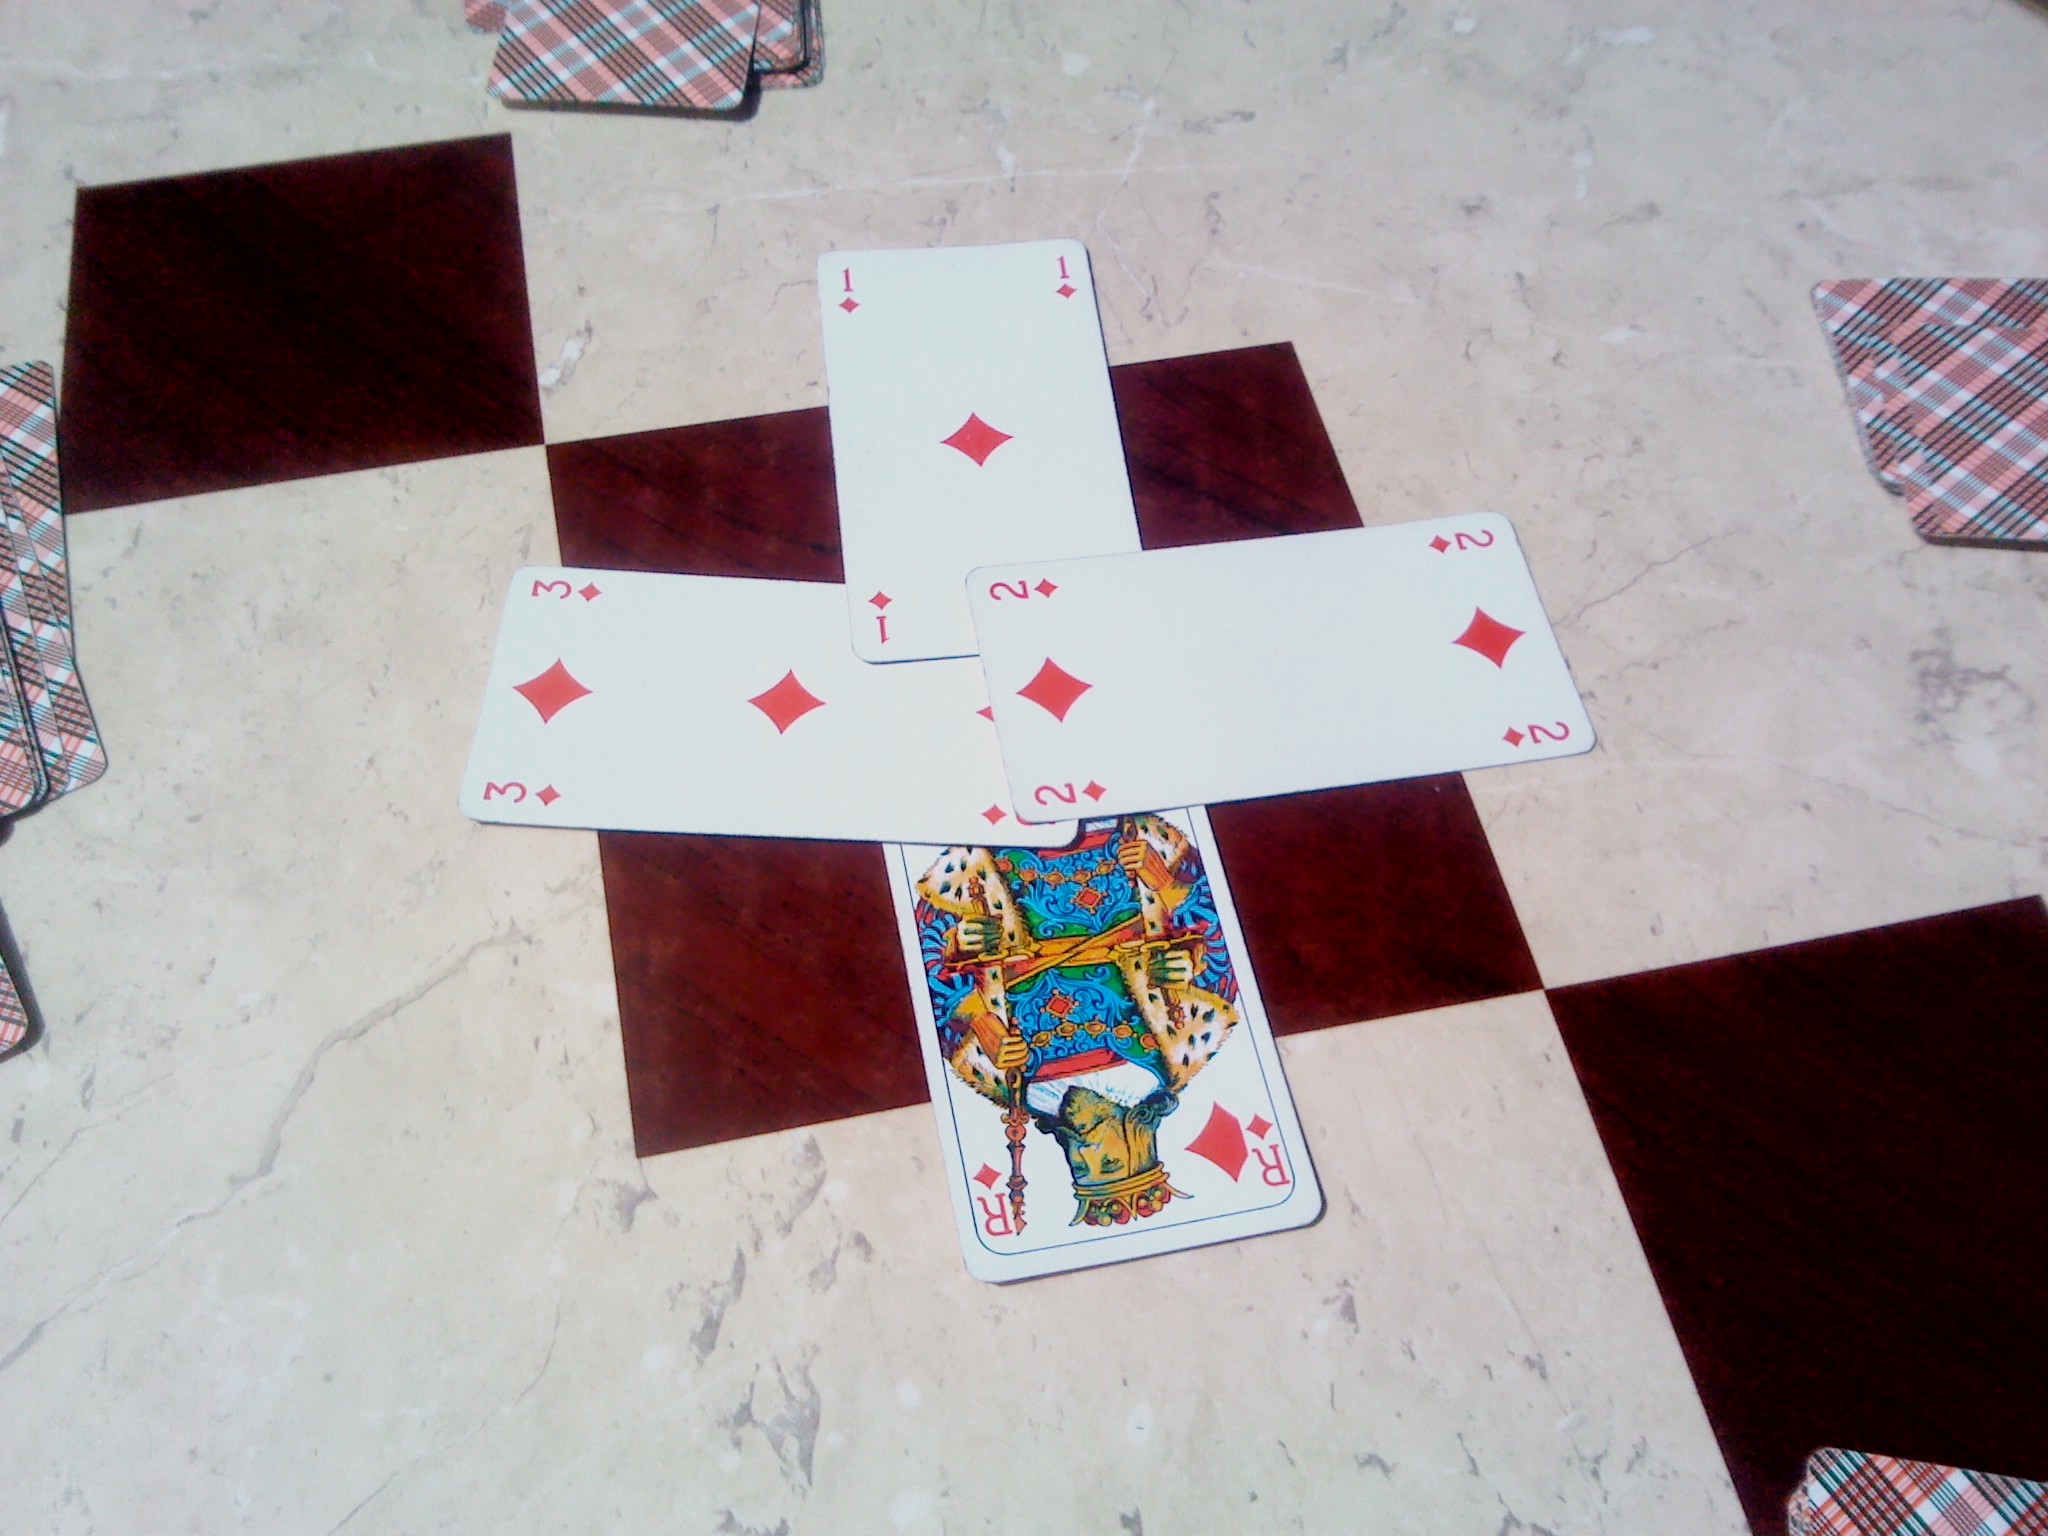
\includegraphics[scale=0.15]{Images/2.jpg}
			\end{center}


	\section{Les scores}
		
		Les scores se calculent de la manière différente suivant les préférences des joueurs.\\
		Il y a deux grandes manières de compter les points qui se démarquent. Une qui est devenue officielle et une qui est restée grandement utilisée.\\
		\\ 
		Il faut savoir que seul le nombre de bouts détermine le nombre de points à réaliser pour remplir le contrat.\\
		En effet à la fin d’une donne on voit combien de bouts a le preneur, et le nombre de points qu’il doit faire pour réussir suit les règles suivantes :\\
		\begin{itemize}
		    \item 3 bouts = 36 points
		    \item 2 bouts = 41 points
		    \item 1 bout = 51 points
		    \item 0 bout = 56 points
		\end{itemize}

		Ce sont les seuils minimum à atteindre pour réussir un contrat. Si le contrat n’est pas réussi on garde la différence, ainsi que lorsque l’on dépasse le seuil on conserve aussi 			la différence.\\

		Exemple :
		\begin{enumerate}

			\item Si un joueur à la fin d’une partie a 2 bouts et 51 points, il a réussi son contrat de 10 points.
		    		(51 - 41)  = 10
			\item Si en revanche il n’avait pas de bout mais le même nombre de points il aurait perdu de 5 points.
		    		(51 - 56) = - 5
		\end{enumerate}
			\subsection{Calcul selon la FFT (Fédération Française de Tarot)}
				Il y a une mise de base de 25 points, ces points sont ajoutés aux points que fait le preneur.\\
			\begin{enumerate}
				\item(10 + 25) = 35
				\item(5 + 25) = 30
			\end{enumerate}

			Ensuite ce total est multiplié par un facteur correspondant au contrat annoncé par le preneur en début de donne.\\
				Voici les différent facteurs :\\
				\begin{itemize}
					\item Petite ou Prise : facteur = 1
				   	\item Garde : facteur = 2
				    	\item Garde Sans : facteur = 4
				    	\item Garde Contre : facteur = 6
				\end{itemize}

				\begin{enumerate}
					\item(30 * 4) = 140
					\item(30 * 1) = 30
				\end{enumerate}

			\subsection{Calcul populaire}

				Cette méthode est plus populaire car beaucoup plus simple. Il n’y a pas de facteur associé aux contrats, seulement la mise de base qui varie en fonction du contrat.\\

				Voici les mises en fonction des contrats :\\
				\begin{itemize}
				    	\item Petite ou Prise : 20
				    	\item Garde : 40
				    	\item Garde Sans : 80
				   	\item Garde Contre : 160
				\end{itemize}


				On obtient alors les scores de la donne suivant un calcul dépendant du nombre de joueurs.\\

				Si le jeu est à 4 joueurs :\\

				Le preneur marque 3 fois son résultat en positif s’il a réussi son contrat, sinon en négatif.\\
				Les trois autres joueurs le marque en négatif si le preneur a réussi son contrat, sinon en positif.\\
ê
				Scores finaux d’une donne
				\begin{enumerate}
					\item  
					\begin{itemize}
						\item pour le preneur : (140 * 3) = +420
				  		\item  pour les autres : - 140
					\end{itemize}
					\item  
					\begin{itemize}
				 		\item pour le preneur : (30 * 3) = 90 donc - 90 car il n’a pas réussi son contrat
				   		\item pour les autres : +30
					\end{itemize}
				\end{enumerate}
				Ensuite pour chaque joueur les scores finaux d’une donne sont ajoutés aux scores de la partie en cours.\\
				\\


				La façon de compter les points de la FFT permet de plus tenir compte des points faits par le preneur mais elle est un peu plus compliquée à calculer.\\
				Tandis que celle utilisée par beaucoup de gens est bien plus simple à calculer.\\
				La version officieuse du calcul des scores permet de faire rapidement les calculs des scores de tête, et évite les confusions lors de l’ajout aux scores précédents.\\
				En effet dans une partie de tarot on fait généralement plusieurs donnes, chaque score est ajouté aux précédents pour savoir à la fin d’une partie qui a gagné. (Celui 					qui gagne n’est donc pas forcément celui qui a remporté le plus de donnes.)\\













\chapter{Cahier des charges}
	\section{Introduction}

		Pour le TER du S6, nous avons proposé d'établir comme projet informatique, le développement d'une application mobile en java sous Android. Cela nous apprendra également d'avoir de plus 			amples 	connaissances sur ce langage et sur la programmation objet.
	\section{Description}

		Cette application Android s'agit d'un jeu de tarot composée d'une intelligence artificielle (pour les joueurs que l'utilisateur va affronter) et d'une interface graphique. Cette 			application sera essentiellement codée en Java. L'interface graphique contiendra du XML et l'intelligence artificielle en Lua.
	\section{Objectifs primaires}

		Ce TER se compose de plusieurs objectifs que nous tenons à respecter :
		\begin{itemize}
			\item L'utilisateur aura la possibilité de pouvoir faire des parties à 4 joueurs.
			\item Un système de comptage de points (scores) sera mis au point.
			\item Une interface de script pour l'intelligence artificielle rédigée exclusivement en Lua.
			\item Une interface graphique Android devra être développée et être la plus simple pour l'utilisateur tout en conservant un certain aspect esthétique.
		\end{itemize}
	\section{Objectifs secondaires}
		\begin{itemize}
			\item Partie à 3 et 5 joueurs
			\item Jeu multijoueur en ligne (Client-Serveur)
			\item Possibilité de changer la façon de jouer des IA
			\item Reprendre une partie sauvegardée
		\end{itemize}
	\section{Syntaxe/Conventions de nommage}

		\subsection{Java :}
			\begin{itemize}
				\item Classe : majuscule puis minuscule et majuscule pour séparer les mots sans espace (Ex : EcranJeu).
				\item Méthodes et variables/attributs : minuscule et majuscule pour separer les mots sans espace (Ex : afficherMain()).
				\item Indentation : Toujours utiliser des accolades, même si il n'y a qu'une instruction dans le for ou le if. Et les placer à la ligne après la dernière ligne de code 					et alignée à la première accolade.
				\item Commentaires : juste après la partie commentée.
			\end{itemize}
		\subsection{Lua :}

		La simplicité de la syntaxe de Lua fait que les conventions d'indentation et retour chariot émergent "naturellement". Retour chariot et indentation après les "then" et  "do", retour 			chariot après chaque instruction, et retour chariot et désindentation après les "end".\\
		Tous les objets et variables sont en minuscules, avec des majuscules en début de mot à partir du deuxieme mot.\\


		\subsection{XML :}

		Après l'ouvrage de balises, il y aura un saut de ligne avec une tabulation. A chaque nouvel attribut on sautera une ligne aussi ou pour fermer la balise.

	\section{Outils}

		Les principaux outils que nous utiliserons sont :
		\begin{itemize}
			\item Environnement de développement Eclipse (Indigo)
			\item ADT Plugin pour Eclipse [inclut AVD ci-dessous]
			\item Gestionnaire de sources SVN Subversion.
			\item Google Docs/Google Code.
			\item Librairie LuaJava (version projet AndroLua) compilée avec Android NDK.
			\item Android SDK Manager.
			\item Android Virtual Device (émulateur Android 2.2).
		\end{itemize}
	\section{UML}
	(voir annexe fournie)











\chapter{État de l'art}
	Android est un système d’exploitation open source utilisant le noyau Linux pour smartphones.\\
	Android est construit sur deux points :\\
	\begin{itemize}
	  	\item Le langage java
	    \item Le SDK qui permet de développer des applications pour mobile
	\end{itemize}
	Le kit de développement donne accès à une documentation complète et à un émulateur.\\
	Android est un système de la famille de Linux. Il s’appuie sur :\\
	\begin{itemize}
	   	\item un noyau Linux
	   	\item une machine virtuelle
	   	\item des applications
	   	\item des bibliothèques
	\end{itemize}

	\section{Découverte d’Android}
		\subsection{Description}
			Android est un système d'exploitation open-source pour smartphones, PDA et autres terminaux mobiles, conçu par Android, une start-up rachetée par Google en juillet 2005. Il 				existe d'autres types d'appareils possédant ce système d'exploitation tels que les téléviseurs et les tablettes.\\
			Le but de cette alliance est de mettre en place des normes ouvertes dans le domaine de la téléphonie mobile. Ce qui veut dire que les développeurs d'application Android pourront 				accéder aux fonctionnalités du cœur de téléphone via une API très fournie.\\
			Android aura comme principaux concurrents Apple avec l'iPhone, Microsoft et son Windows	Mobile et Nokia avec Symbian.\\

		\subsection{Les versions d’Android}
			\begin{center}
				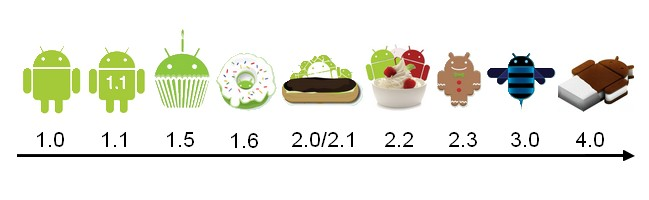
\includegraphics[scale=0.7]{Images/versionsandroid.jpg}
			\end{center}
			L'historique des versions d'Android a débuté avec la sortie de la version 1.0 en septembre 2008. Android a connu plusieurs mises à jour depuis sa première version. Ces mises à 			jour servent généralement à corriger des bugs et à ajouter de nouvelles fonctionnalités. Dans l'ensemble, chaque version est développée sous un nom de code basé sur des 				desserts.	\\
			En octobre 2008, apparait la première version d'Android qui n'avait pas reçu de nom. Cette version s'est avérée être la beta du système.
			La version 1.5 Cupcake corrigea le manque d'API et rendit le système plus utilisable.\\
			Depuis, Android 1.6, 2.0 et 2.1 ont apporté d'importantes améliorations respectivement sur les
			fonctionnalités et sur l'interface graphique du système.\\
			Android 3.0 est spécifique aux tablettes. Android 4.0 est la dernière version en date qui apporte de nombreuses fonctionnalités et est compatible aussi bien sur les smartphones 				que sur les tablettes.\\
		
		\subsection{Fonctionnalités d’Android}
			\subsubsection{Les éléments d’une application}
				Une application Android est composée des éléments suivants:\\
				\begin{itemize}
					\item des activités (android.app.Activity) : il s'agit d'une partie de l'application présentant une vue à l'utilisateur
					\item des services (android.app.Service) : il s'agit d'une activité tâche de fond sans vue associée
					\item des fournisseurs de contenus (android.content.ContentProvider): permet le partage d'informations au sein ou entre applications
					\item des widgets (android.appwidget.*) : une vue accrochée au Bureau d'Android
					\item des Intents (android.content.Intent) : permet d'envoyer un message pour un composant externe sans le nommer explicitement
					\item des récepteurs d'Intents (android.content.BroadcastReceiver) : permet de déclarer être capable de répondre à des Intents
					\item des notifications (android.app.Notifications) : permet de notifier l'utilisateur de la survenue d'événements
				\end{itemize}
			
			\subsubsection{Le manifest}
				Le fichier AndroidManifest.xml déclare l'ensemble des éléments de l'application :\\
				\begin{verbatim}
				<?xml version="1.0" encoding="utf-8"?>
				<manifest xmlns:android="http://schemas.android.com/apk/res/android"
				   package="fr.apln.TutoAndroid\_1"
				   android:versionCode="1"
				   android:versionName="1.0" >

				   <uses-sdk android:minSdkVersion="8" />

				   <application
				       android:icon="@drawable/ic_launcher"
				       android:label="@string/app_name" >
				       <activity
					   android:name=".TutoAndroid_1"
					   android:label="@string/app_name" >
					   <intent-filter>
					       <action android:name="android.intent.action.MAIN" />
						
					       <category android:name="android.intent.category.LAUNCHER" />
					   </intent-filter>
				       </activity>
				   </application>
				</manifest>
				\end{verbatim}
			\subsubsection{Les ressources}
				Les ressources de l'applications sont utilisées dans le code au travers de la classe statique R. ADT re-génère automatiquement la classe statique R à chaque changement 				dans le projet. Toutes les ressources sont accessibles au travers de R, dés qu'elles sont déclarées dans le fichier XML ou que le fichier associé est déposé dans le 					répertoire adéquat. Les ressources sont utilisées de la manière suivante:\\

				android.R.type\_ressource.nom\_ressource\\

				qui est de type int. Il s'agit en fait de l'identifiant de la ressource. On peut alors utiliser cet identifiant ou récupérer l'instance de la ressource en utilisant la 				classe Resources:\\

				Resources res = getResources();\\
				String hw = res.getString(R.string.hello);\\
				XXX o = res.getXXX(id);\\

				Une méthode spécifique pour les objets graphiques permet de les récupérer à partir de leur id, ce qui permet d'agir sur ces instances même si elles ont été créées via 					leur définition XML:\\

				TextView texte = (TextView)findViewById(R.id.le\_texte);\\
				texte.setText("Here we go !");\\
		\subsection{Architecture}
			Le diagramme suivant illustre les composants principaux du système d’exploitation Android :\\
			\begin{center}
				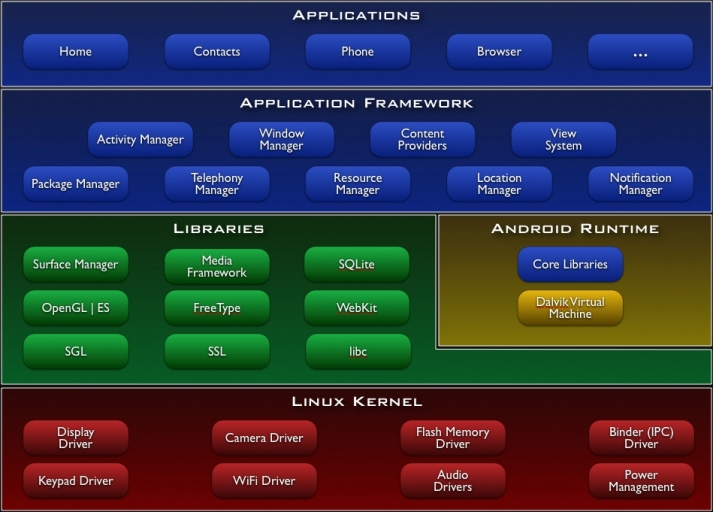
\includegraphics[scale=0.5]{Images/architecture-systeme-android.jpg}
			\end{center}
			Android est basé sur un kernel linux 2.6.xx.\\
			Au-dessus de cette couche, on retrouve les librairies C/C++ utilisées par un certain nombre de
			composants du système Android.\\
			Au-dessus des librairies, on retrouve l'Android Runtime. Cette couche contient les librairies cœurs
			du Framework ainsi que la machine virtuelle exécutant les applications.\\
			Au-dessus de la couche "Android Runtime" et des librairies cœurs, on retrouve le Framework
			permettant au développeur de créer des applications. Enfin au-dessus du Framework, il y a les
			applications.\\
	
	\section{Réalisation d’un projet Android}
		\subsection{Le SDK}
			Basé sur le langage Java, le SDK Android nécessite d'avoir un JDK (5 ou 6) installé sur sa machine pour pouvoir être utilisé.\\

			Un projet basé sur le plugin ADT est décomposé de la manière suivante :\\
			
			\begin{itemize}
			    	\item src/: les sources Java du projet
			    	\item libs/: bibliothèques tierces
			    	\item res/:
				\begin{itemize}
					\item res/drawable: ressources images
					\item res/layout: description des IHMs en XML
					\item res/values: chaines de caractères et dimensions
				\end{itemize}
			    	\item gen/: les ressources auto générées par ADT
			    	\item assets/: ressources brutes (raw bytes)
			    	\item bin/:
				\begin{itemize}
					\item bin/classes: les classes compilées en .class
					\item bin/classes.dex: exécutable pour la JVM Dalvik
					\item bin/myapp.zip: les ressources de l'application
					\item bin/myapp.apk: application empaquetée avec ses ressource et prête pour le déploiement		
				\end{itemize}
			\end{itemize}

	\section{Création d’un projet Android}
		\subsection{Activité}
			Une activité correspond à un écran. Si une application se compose de plusieurs écrans, elle a une activité pour chaque écran. Chaque activité est une classe qui étend la classe 				de base Activity. Elle dispose d'une interface utilisateur graphique faite de vues (views) et elle répond à des évènements (events). Quand on change d'écran, on lance une 				nouvelle activité.\\

			Une activité n'a pas de contrôle direct sur son propre état, il s'agit plutôt d'un cycle rythmé par les interactions avec le système et d'autres applications. Voici un schéma 				explicatif du cycle de vie d’une activité : \\
			\begin{center}
				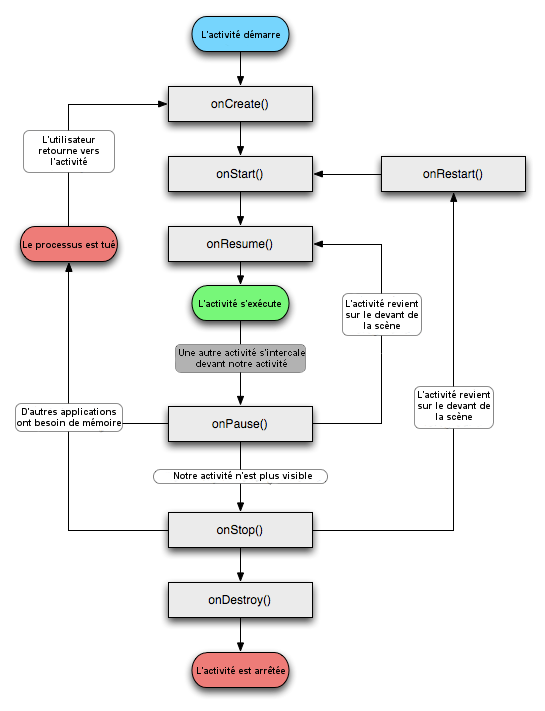
\includegraphics[scale=0.5]{Images/activ.png}
			\end{center}
			


		\subsection{Création du projet}
			L’assistant de création permet de facilement créer un nouveau projet Android.\\


			\begin{center}
				
\includegraphics[scale=0.5]{Images/un.png}
			\end{center}
			La nouvelle fenêtre permet de donner un nom au projet ainsi que son emplacement : \\

			\begin{center}
				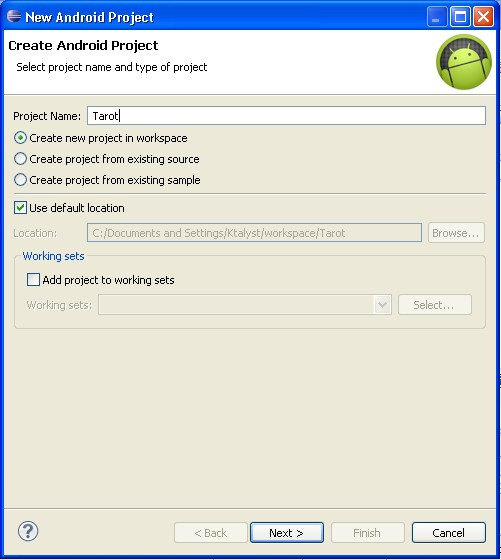
\includegraphics[scale=0.5]{Images/deux.jpg}
			\end{center}

			L’écran suivant permet de sélectionner la version d’Android pour laquelle sera compilé le projet.\\
			Puis le dernier écran permet de choisir le nom de l’application, le package, et la version minimum du SDK acceptée. A partir de là, on peut enfin commencer à écrire une vraie 				application !\\

			\begin{center}
				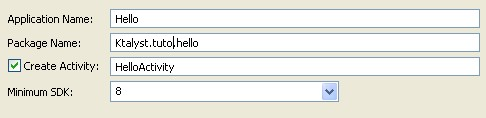
\includegraphics[scale=0.5]{Images/trois.jpg}
			\end{center}
		\subsection{Hello world}
			
			Dans le répertoire /src, on retrouve les classes .java. Le fichier HelloActivity contient alors :\\
			\begin{verbatim}
			package sdz.chapitreUn.preums;

			import android.app.Activity;

			import android.os.Bundle;

			public class HelloActivity extends Activity {

			   @Override

			   public void onCreate(Bundle savedInstanceState) {

			       super.onCreate(savedInstanceState);

			       setContentView(R.layout.main);

			   }

			}
			\end{verbatim}
			On reconnait le package choisi un peu plus tôt et les deux classes dont nous avons besoin pour créer notre application : Activity et Bundle.\\

			L’activité hérite de la classe Activity et l’Override permet d’indiquer que l’on va redéfinir une méthode appartenant à la classe Activity.\\

			La méthode onCreate(...) est la première qui est lancée au démarrage d'une application. super.onCreate fait appel au onCreate de la classe Activity.\\

			Et pour afficher notre “Hello World”, nous allons faire appel à un attribut de type TextView. Nous nous retrouvons donc avec :\\
			\begin{verbatim}
			import android.app.Activity;
			import android.os.Bundle;
			import android.widget.TextView;

			public class Hello Activity extends Activity {
			   TextView hello = null;

			   @Override
			   public void onCreate(Bundle savedInstanceState)
			   {
			       super.onCreate(savedInstanceState);
			       
			       hello = new TextView(this);
			       hello.setText("Hello world");
			       setContentView(hello);
			   }
			}

			La méthode void setContentView permet d’afficher à l’écran la vue passée en paramêtre. 
			\end{verbatim}
		\subsection{Interface graphique}
			Les éléments graphiques héritent de la classe View. Chaque partie de notre interface est une vue ou un groupe de vues qui hérite de cette classe. Une vue est un widget qui a une 				apparence à l’écran : label, boutons, … Les vues peuvent être regroupées ainsi :\\
			\begin{center}
				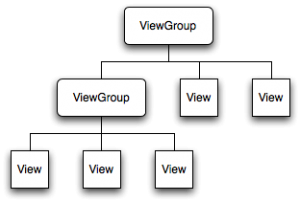
\includegraphics[scale=0.5]{Images/viewgroup.png}
			\end{center}
			Ces groupes de vues sont utilisés pour gérer la mise en page des interfaces graphiques.\\

			La notion de mise en page est reliée à la notion de "Layout". Cette dernière représente l'agencement des différents éléments graphiques dans votre interface. Par exemple, le 				LinearLayout permet d’organiser les éléments sur une ligne ou colonne. Les déclarations se font principalement en XML.\\
			\begin{verbatim}
			<LinearLayout xmlns:android="http://schemas.android.com/apk/res/android"
			 android:orientation="vertical"
			 android:layout_width="fill_parent"
			 android:layout_height="fill_parent"
			 android:gravity="center"
			 android:id="@+id/accueilid"
			 >
			</LinearLayout>
			\end{verbatim}
			\begin{itemize}
				\item android :orientation : définit l'orientation
	  			\item android:gravity : définit l'alignement des éléments
				\item android:layout\_width="fill\_parent" : l'élément remplit tout l'élément parent
			\end{itemize}



	\section{Réalisation d’un projet Android}
		\subsection{Le SDK}
			Basé sur le langage Java, le SDK Android nécessite d'avoir un JDK (5 ou 6) installé sur sa machine pour pouvoir être utilisé.\\

			Un projet basé sur le plugin ADT est décomposé de la manière suivante :\\
			
			\begin{itemize}
			    	\item src/: les sources Java du projet
			    	\item libs/: bibliothèques tierces
			    	\item res/:
				\begin{itemize}
					\item res/drawable: ressources images
					\item res/layout: description des IHMs en XML
					\item res/values: chaines de caractères et dimensions
				\end{itemize}
			    	\item gen/: les ressources auto générées par ADT
			    	\item assets/: ressources brutes (raw bytes)
			    	\item bin/:
				\begin{itemize}
					\item bin/classes: les classes compilées en .class
					\item bin/classes.dex: exécutable pour la JVM Dalvik
					\item bin/myapp.zip: les ressources de l'application
					\item bin/myapp.apk: application empaquetée avec ses ressource et prête pour le déploiement		
				\end{itemize}
			\end{itemize}

	\section{Création d’un projet Android}
		\subsection{Activité}
			Une activité correspond à un écran. Si une application se compose de plusieurs écrans, elle a une activité pour chaque écran. Chaque activité est une classe qui étend la classe 				de base Activity. Elle dispose d'une interface utilisateur graphique faite de vues (views) et elle répond à des évènements (events). Quand on change d'écran, on lance une 				nouvelle activité.\\

			Une activité n'a pas de contrôle direct sur son propre état, il s'agit plutôt d'un cycle rythmé par les interactions avec le système et d'autres applications. Voici un schéma 				explicatif du cycle de vie d’une activité : \\
			\begin{center}
				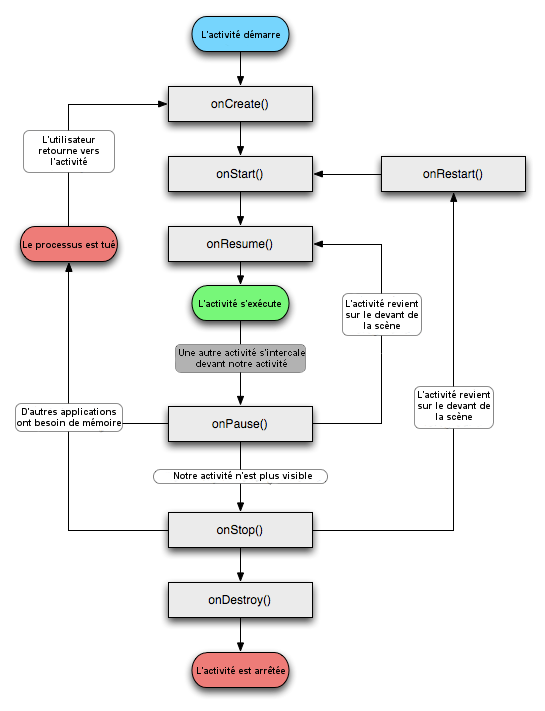
\includegraphics[scale=0.5]{Images/activ.png}
			\end{center}
			


		\subsection{Création du projet}
			L’assistant de création permet de facilement créer un nouveau projet Android.\\


			\begin{center}
				
\includegraphics[scale=0.5]{Images/un.png}
			\end{center}
			La nouvelle fenêtre permet de donner un nom au projet ainsi que son emplacement : \\

			\begin{center}
				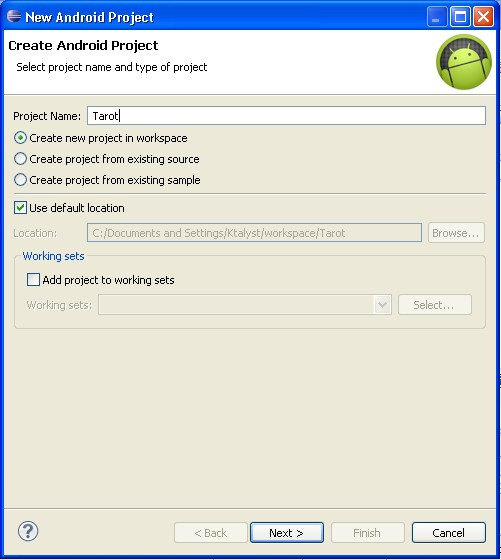
\includegraphics[scale=0.5]{Images/deux.jpg}
			\end{center}

			L’écran suivant permet de sélectionner la version d’Android pour laquelle sera compilé le projet.\\
			Puis le dernier écran permet de choisir le nom de l’application, le package, et la version minimum du SDK acceptée. A partir de là, on peut enfin commencer à écrire une vraie 				application !\\

			\begin{center}
				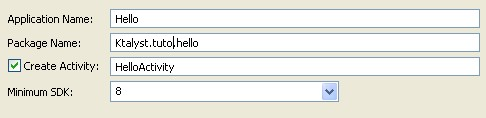
\includegraphics[scale=0.5]{Images/trois.jpg}
			\end{center}
		\subsection{Hello world}
			
			Dans le répertoire /src, on retrouve les classes .java. Le fichier HelloActivity contient alors :\\
			\begin{verbatim}
			package sdz.chapitreUn.preums;

			import android.app.Activity;

			import android.os.Bundle;

			public class HelloActivity extends Activity {

			   @Override

			   public void onCreate(Bundle savedInstanceState) {

			       super.onCreate(savedInstanceState);

			       setContentView(R.layout.main);

			   }

			}
			\end{verbatim}
			On reconnait le package choisi un peu plus tôt et les deux classes dont nous avons besoin pour créer notre application : Activity et Bundle.\\

			L’activité hérite de la classe Activity et l’Override permet d’indiquer que l’on va redéfinir une méthode appartenant à la classe Activity.\\

			La méthode onCreate(...) est la première qui est lancée au démarrage d'une application. super.onCreate fait appel au onCreate de la classe Activity.\\

			Et pour afficher notre “Hello World”, nous allons faire appel à un attribut de type TextView. Nous nous retrouvons donc avec :\\
			\begin{verbatim}
			import android.app.Activity;
			import android.os.Bundle;
			import android.widget.TextView;

			public class Hello Activity extends Activity {
			   TextView hello = null;

			   @Override
			   public void onCreate(Bundle savedInstanceState)
			   {
			       super.onCreate(savedInstanceState);
			       
			       hello = new TextView(this);
			       hello.setText("Hello world");
			       setContentView(hello);
			   }
			}

			La méthode void setContentView permet d’afficher à l’écran la vue passée en paramêtre. 
			\end{verbatim}
		\subsection{Interface graphique}
			Les éléments graphiques héritent de la classe View. Chaque partie de notre interface est une vue ou un groupe de vues qui hérite de cette classe. Une vue est un widget qui a une 				apparence à l’écran : label, boutons, … Les vues peuvent être regroupées ainsi :\\
			\begin{center}
				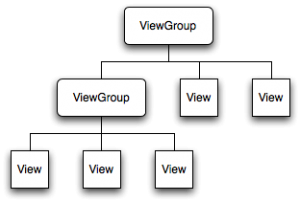
\includegraphics[scale=0.5]{Images/viewgroup.png}
			\end{center}
			Ces groupes de vues sont utilisés pour gérer la mise en page des interfaces graphiques.\\

			La notion de mise en page est reliée à la notion de "Layout". Cette dernière représente l'agencement des différents éléments graphiques dans votre interface. Par exemple, le 				LinearLayout permet d’organiser les éléments sur une ligne ou colonne. Les déclarations se font principalement en XML.\\
			\begin{verbatim}
			<LinearLayout xmlns:android="http://schemas.android.com/apk/res/android"
			 android:orientation="vertical"
			 android:layout_width="fill_parent"
			 android:layout_height="fill_parent"
			 android:gravity="center"
			 android:id="@+id/accueilid"
			 >
			</LinearLayout>
			\end{verbatim}
			\begin{itemize}
				\item android :orientation: définit l'orientation
	  			\item android:gravity : définit l'alignement des éléments
				\item android:layout\_width="fill\_parent" : l'élément remplit tout l'élément parent
			\end{itemize}







\chapter{Organisation du projet}
	\section{Organisation du travail}


		La première étape fût de nous réunir une première fois en début de semestre afin de bien cibler la chronologie des tâches à effectuer. De ce fait, le groupe avait déjà commencer à 			implémenter le jeu en “mode texte” (créations de classes en Java) car il nous fallait en quelque sorte une base pour que le groupe puisse déterminer ensuite qui devait travailler sur 			quoi plus précisément. Une fois que cela a été fait, une autre réunion s’est déroulée pour répartir la suite du travail (en sous-groupe éventuellement).\\
		\\ 
		La répartition des tâches était la suivante :\\
		\begin{itemize}
			\item L’ interface graphique et son implémentation fonctionnelle : Sylvain Brunerie, Jennifer Roudet, Heykel Hachiche.
			\item Le moteur de jeu : Fabrice Thill, Jean-Baptiste Subils, Sylvain Brunerie.
			\item Intelligence artificielle : Kevin Bradshaw, Jean-Baptiste Subils.
			\item Réseau : Fabrice Thill, Jean-Baptiste Subils, Sylvain Brunerie.
		\end{itemize}
	
	\section{Choix des outils}
		Le langage Java nous étant imposé* par le choix de la plateforme Android, nous avons décidé de travailler en utilisant l’environnement de développement Eclipse. Les raisons de ce choix 			sont multiples : c’est un IDE que nous connaissons plutôt bien, il est libre et gratuit. Mais surtout, dans le cadre de la programmation Android, il est presque incontournable car 		il permet d’utiliser le plugin ADT (Android Development Tools), qui fournit un certain nombre d’outils, tels que les éditeurs de fichiers XML d’interface, d’internationalisation, de 			préférences…), et la possibilité de lancer l’application dans un émulateur sur l’ordinateur, comme sur un appareil Android physique (connecté à l’ordinateur par liaison USB). Ce plugin est aussi disponible pour Code::Blocks et NetBeans, mais l’intégration est encore expérimentale et incomplète.\\
		Malgré les défauts d’Eclipse (lenteur et lourde empreinte mémoire) et certains comportements parfois agaçants (compilation permanente, qui induit le signalement d’erreurs ou d’avertissements 		pendant l’écriture), il nous a fait économiser beaucoup de temps et d’énergie.\\

		Pour travailler à six étudiants sur le même projet, il n’était pas concevable de travailler chacun de notre côté et d’envoyer les modifications effectuées par e-mail. Nous avons donc 			décidé d’utiliser un système de gestion de versions. Notre choix s’est porté sur Subversion (SVN), que certains d’entre nous connaissaient déjà, et la solution qui est apparue la plus 		simple était la plateforme d’hébergement de projets Google Code, qui offre de nombreux outils, dont un SVN, un wiki et un logiciel de gestion de bugs. Nous n’avons cependant utilisé que 			le SVN.\\

		Pour faciliter les communications entre les différents membres du groupe, nous avons d’abord créé un forum sous phpBB, que nous n’avons finalement pas utilisé, ou presque. L’utilisation 			d’une liste de diffusion (mailing-list) s’est révélée plus efficace. Pour cela, Google nous a une fois de plus apporté le service adapté : Google Groupes.\\
















\chapter{Développement}
	\section{Moteur de jeu}
		
		
		\subsection{Déroulement d'une partie}
			Voici comment se déroule une partie de Tarot dans notre programme.
			\subsubsection{Structure globale d’une partie de tarot}
				La partie de tarot est composée de plusieurs donnes. Elle s’arrête, selon les préférences choisies, au bout d’un certain nombre de donnes ou bien quand un des joueurs a 					atteint un certain score.\\
				Les différentes étapes d’une partie sont explicitées dans le diagramme d’activités de la page suivante.
			\begin{center}
				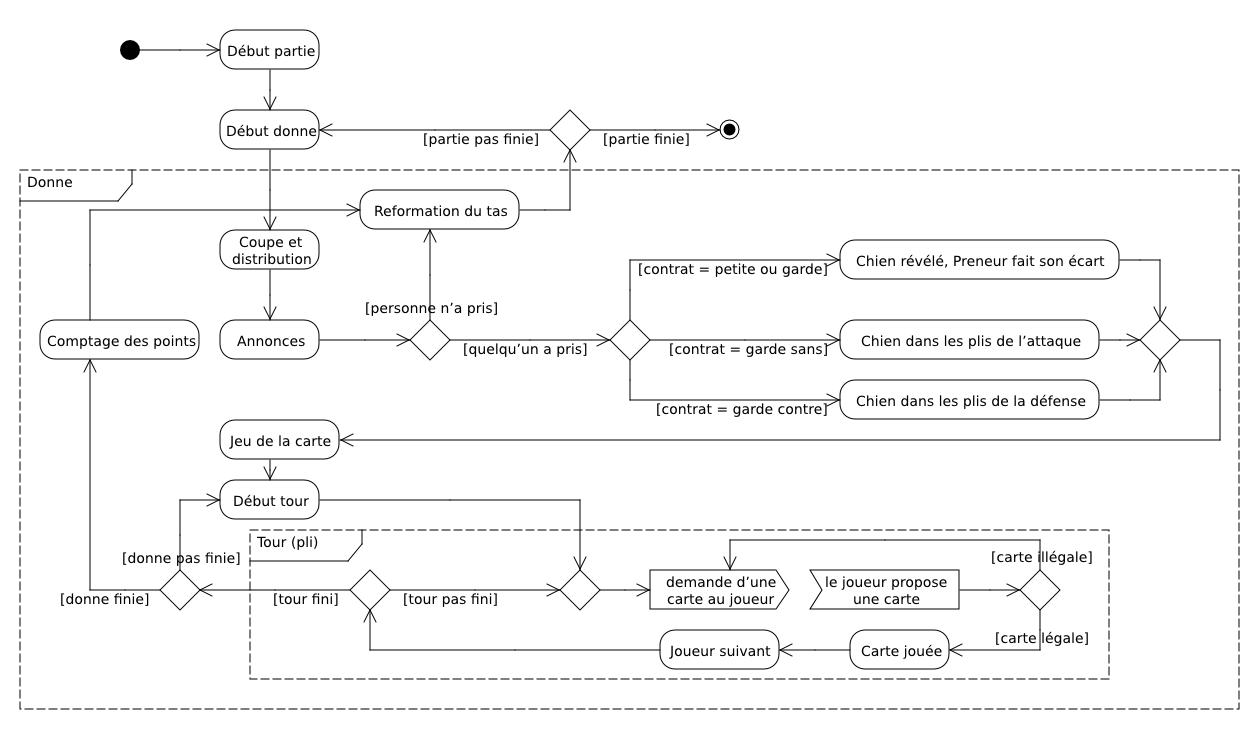
\includegraphics[scale=0.52,angle=90]{Images/flow.jpg}
			\end{center}
			
			\subsubsection{La coupe}	
				Au tarot, on ne mélange pas les cartes entre les donnes. À la fin d’une donne, les plis de l’attaque et les plis de la défense sont regroupés ; cela permet de garder une 					certaine irrégularité qui favorise les contrastes entre les mains des joueurs. Il vaut mieux un joueur avec une très bonne main que quatre joueurs avec des mains pas 					assez fortes pour annoncer un contrat. Au lieu d’un mélange du tas de cartes, pour ne pas que l’on puisse savoir quelles cartes reviennent à quel joueur, le jeu est « 					coupé », c’est-à-dire qu’il est partagé en deux, par la personne située avant le donneur.\\
					Nous avons voulu reproduire cette particularité. Le tas de cartes n’est donc jamais mélangé, et une coupe est effectuée par le programme. Pour représenter au 					mieux les coupes que fait un joueur humain, l’emplacement de celle-ci est déterminée aléatoirement suivant une loi normale gaussienne. En effet, la coupe est la plupart 					du temps effectuée vers le milieu du paquet, bien plus rarement vers les extrémités.\\
				\newpage
			\subsubsection{La distribution des cartes}


				\begin{algorithm}[t!]
				\caption{Algorithme de distribution \label{algodistribution}}
				\KwData{les mains des joueurs $main$ , le tas de cartes $tas$, $NP$ le nombre de cartes pout le chien et les constantes $NT$ pour le nombre de cartes totales et $CD$ le 					nombre de cartes distribues par joueurs }
					\KwResult{Distribution de 78 cartes entre les joueurs}
					 \Begin
					{
						 incrementerNumDonneur();\\ 
						%\tcc{on commence au joueur après le donneur}
						 entier randomMin $\leftarrow$ 1;\\
						 entier j$\leftarrow$ 0\\
						 entier k$\leftarrow$ 0 \\
						 entier CartesAuChien $\leftarrow$ 0;\\

						 
						 possibilitesMisesAuChien := (( NT - NP ) / CD) ;\\
						 \While{( NP - CartesAuChien ) != 0}
						 {
							 randomMax $\leftarrow$ possibilitesMisesAuChien - ( NP - CartesAuChien );\\
							 

							 entier random := randomMin + (int)(Math.random() * ((randomMax - randomMin)+1));\\
							% \tcc{il faut que la valeur de retour soit comprise entre ]randomMin,randomMax] }
							 \While{j<=(random*CD)}
							 {
								 main[numeroDuJoueur] $\leftarrow$ tas.prendrecarte();\\
								 main[numeroDuJoueur] $\leftarrow$ tas.prendrecarte();\\
								 main[numeroDuJoueur] $\leftarrow$ tas.prendrecarte();\\
								 j += 3;\\
								 
								 main[numeroDuJoueur] $\leftarrow$ tas.prendrecarte();\\
							 }
							chien.add(k, P.prendreCarteDuTas());\\
							CartesAuChien++;\\
							j++;\\
							k++;\\
							randomMin := random+1;\\
						}
						 \While{j<NT-1}
						 {
							 main[numeroDuJoueur] $\leftarrow$ tas.prendrecarte();\\
							 main[numeroDuJoueur] $\leftarrow$ tas.prendrecarte();\\
							 main[numeroDuJoueur] $\leftarrow$ tas.prendrecarte();\\
							 j += 3;\\
							 main[numeroDuJoueur] $\leftarrow$ tas.prendrecarte();\\
						 }
						 \ForEach{i de 1 a nombredeJoueurs}
						 {
							 P.getJoueur(i).direMain(mainsDesJoueurs[i].getCartes());\\
						 }
					}
				\end{algorithm}
				\newpage
				Pour la distribution des cartes, nous avons voulu respecter la façon dont les cartes sont distribuées au tarot. En effet, les cartes sont distribuées aux joueurs par 					groupes de 3, et entre ceux-ci de temps en temps des cartes sont mises au chien. Elles doivent être au nombre de six (à quatre joueurs) avant la fin de la distribution.
				Le choix des cartes mises au chien est fait aléatoirement, suivant ainsi un algorithme qui est détaillé ci-dessus.
				\begin{center}
					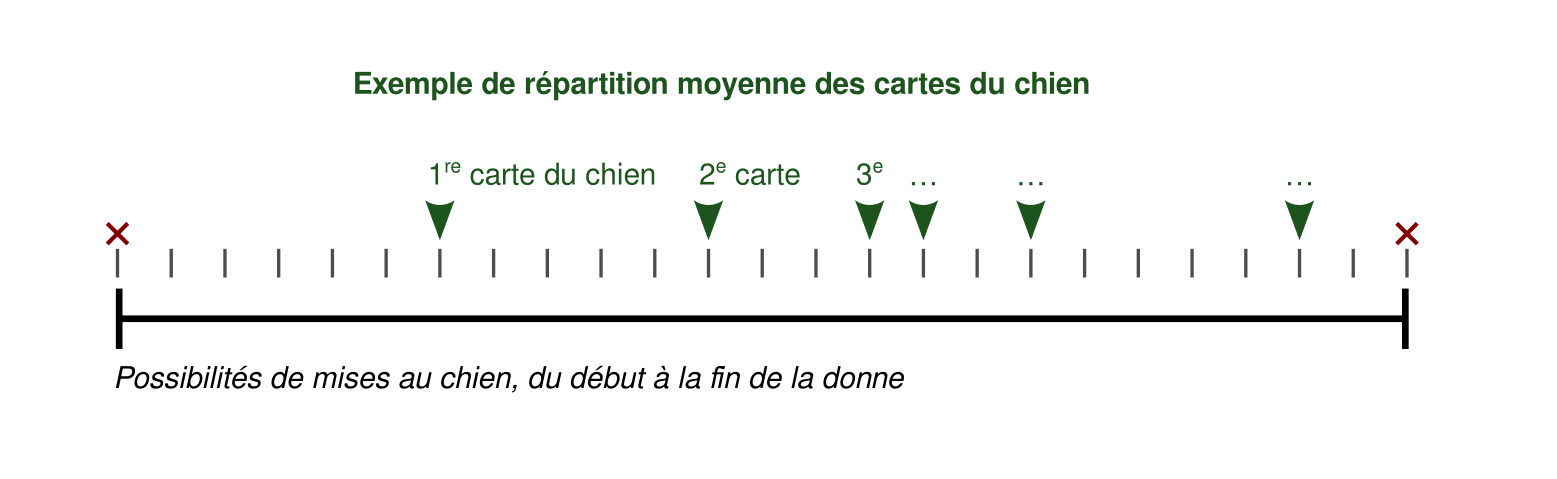
\includegraphics[scale=0.9]{Images/rep.png}
				\end{center}
				Les joueurs n’ont aucune influence sur la distribution, mais les cartes sont tout de même distribuées à partir d’une position et le premier à commencer l’annonce sera un 					joueur ayant une position adjacente.
				Nous avons fait le choix d’automatiser la distribution car la distribution d’un grand nombre de cartes sur un petit écran peut rapidement devenir très frustrant et 					n’apporte rien au jeu de tarot. Une fois les mains et le chien faits, on les donnent au joueurs et on passe à la phase d’annonces.


		\subsection{Communications et généricité : le Croupier}
			Le moteur de jeu communique avec le joueur grâce à la classe ;Croupier, qui se charge de la communication. De cette façon un jeu de tarot peut être lancé avec des types de 				joueurs différents et il est facile car on a pu implémenter le joueur de façon complètement indépendante au moteur de jeu. Le premier type de joueur que nous avons développé 			est une classe JoueurTexte. Celle-ci nous permettait de faire le test du moteur avec une entrée clavier et une sortie écran.
			Ensuite on a le joueur graphique qui permet d'offrir une interface graphique à une personne sur Android et le joueur IA qui est une intelligence artificielle qui joue au tarot.
				\begin{center}
					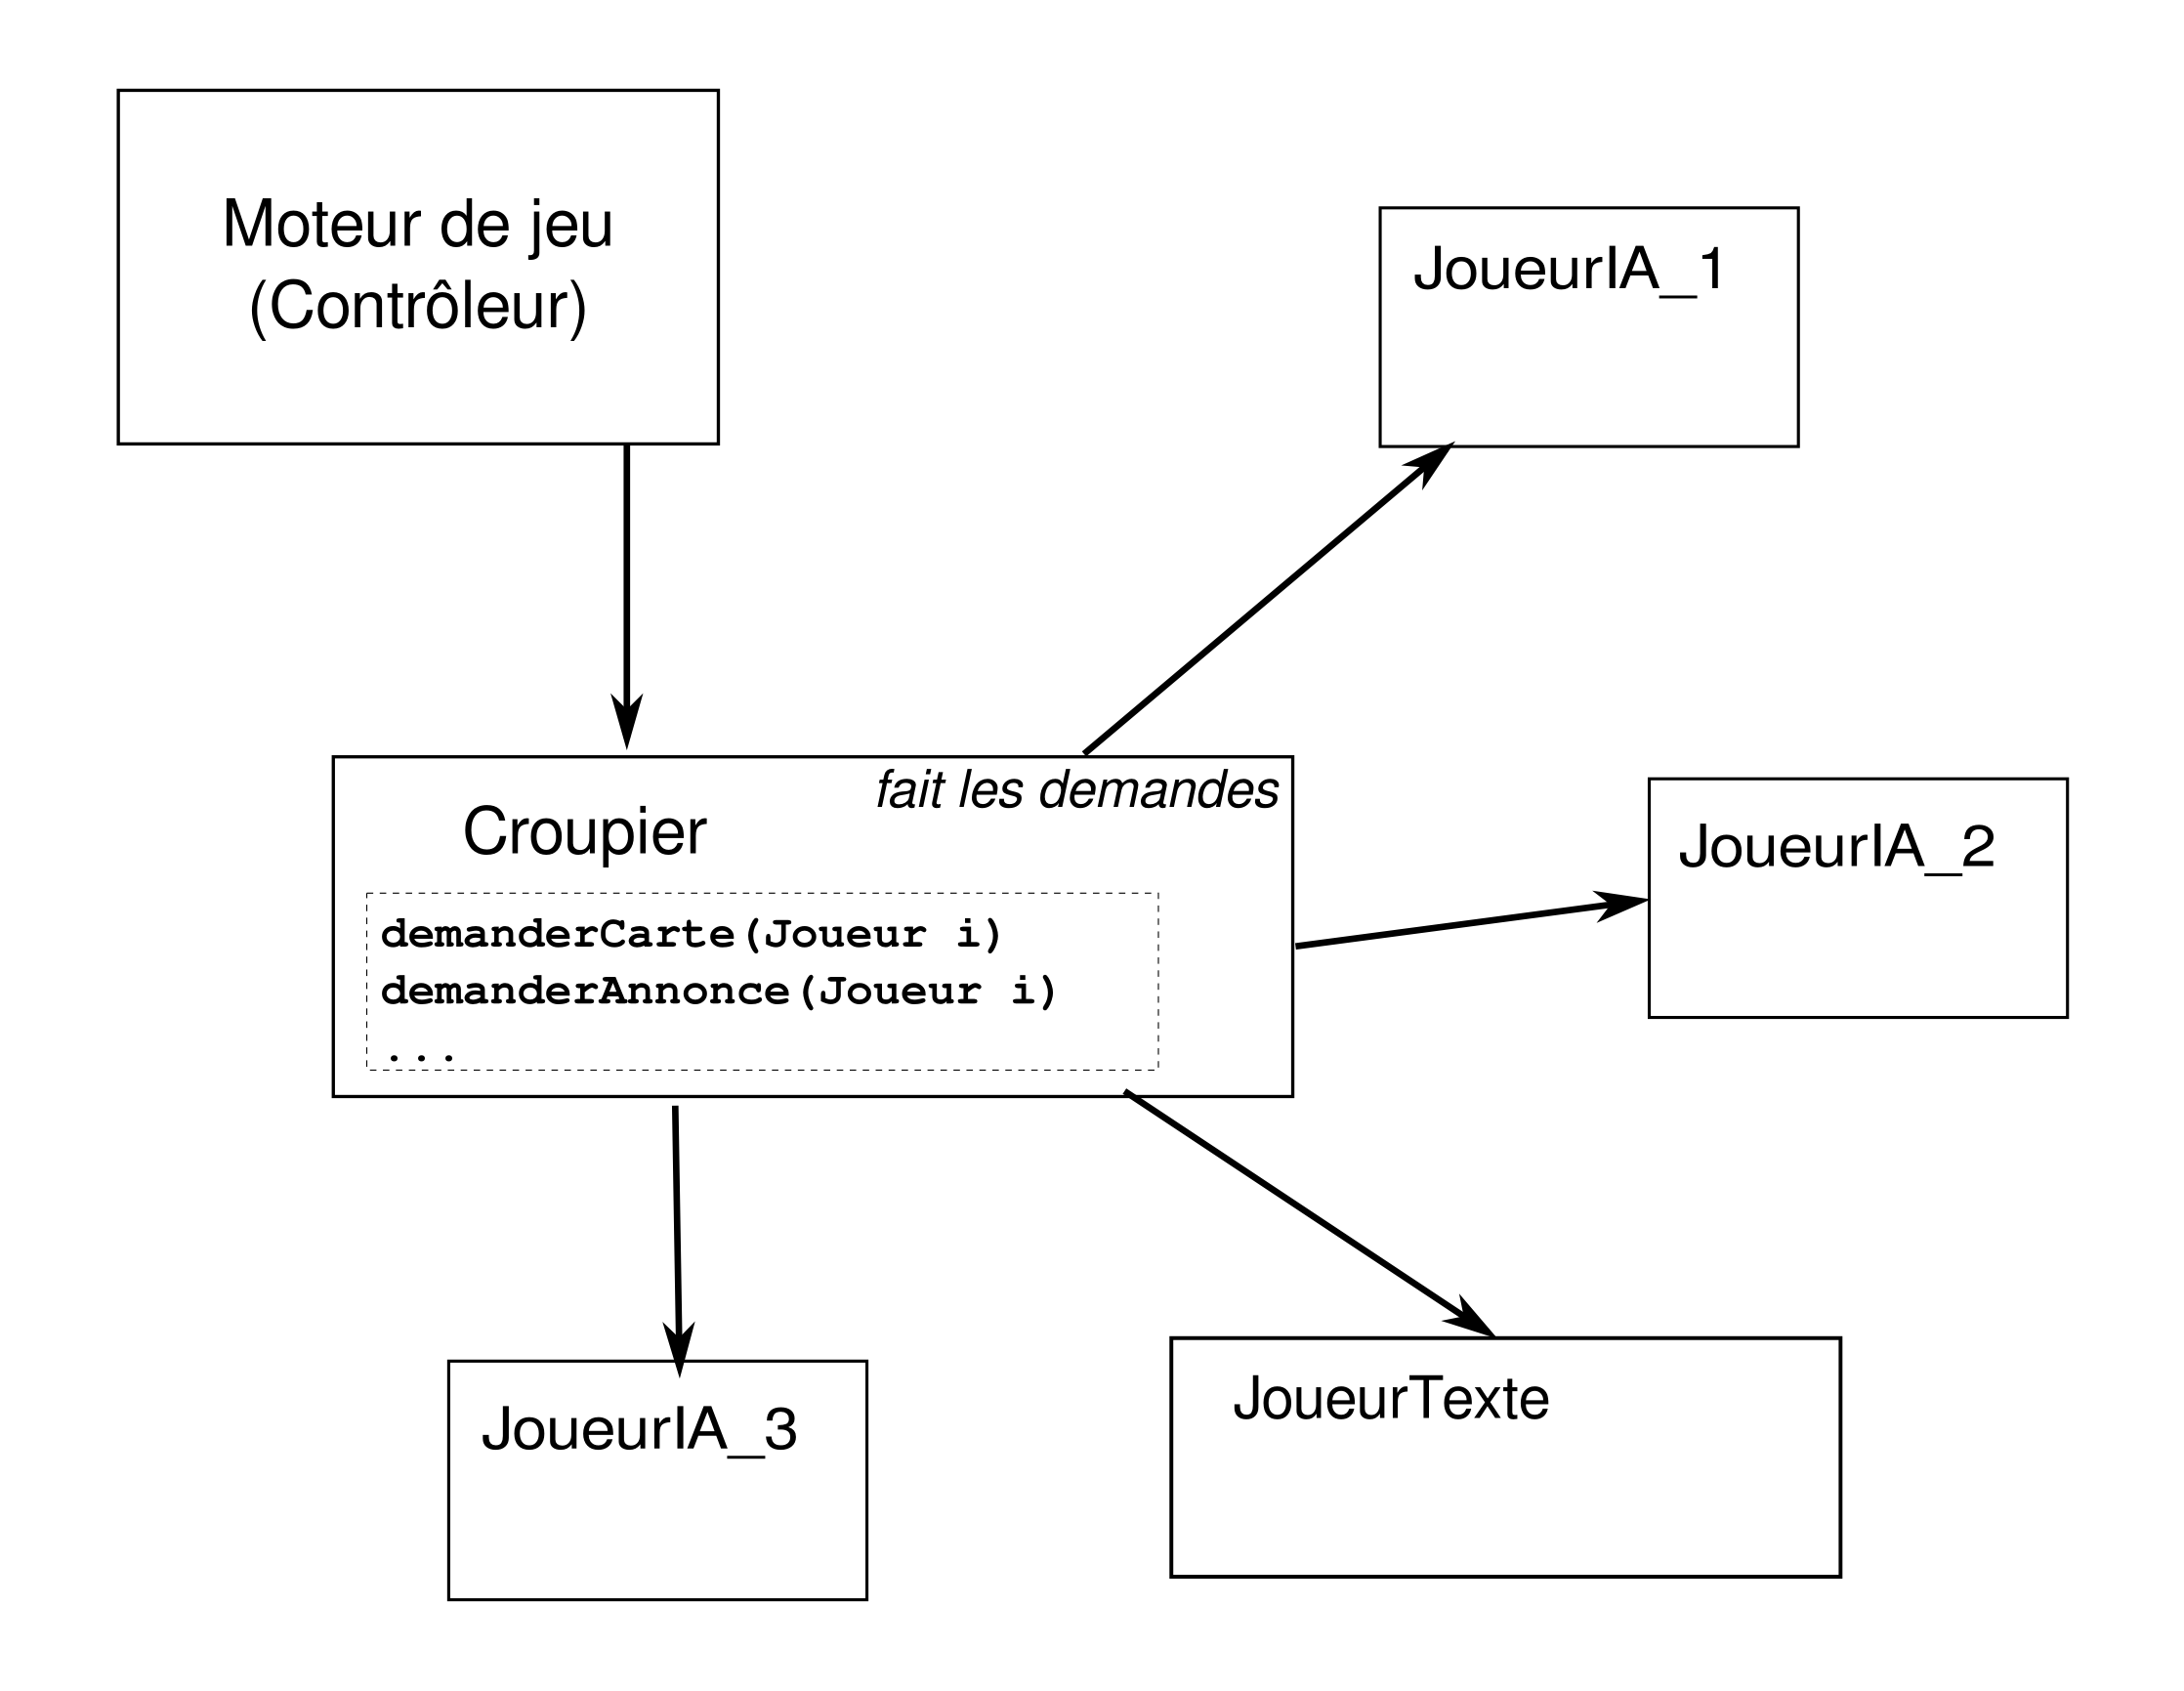
\includegraphics[scale=0.7]{Images/croupier.png}
				\end{center}
			Le développement du moteur même s'est fait de façon assez intuitive. Comme on peut le voir sur le flowchart, une fois une partie lancée, on entre dans une boucle, a l'intérieur 				de laquelle on retrouve une fonction qui se charge de la distribution de cartes, suivi d'une phase d'annonces, une phase de jeu et une phase de score.
			La phase annonce se charge de gérer les annonces. Nous avons fait le choix de traiter la passe comme une annonce de plus bas niveau. La phase annonce s’assure que toute annonce 				faite est légale c'est-à-dire que toute nouvelle annonce est plus forte que les annonces précédentes, la seule exception étant l'annonce passe.
			Une fois que tout le monde a fait son annonce et que personne ne surenchérit, celui qui a l'annonce la plus forte devient preneur. S'il a fait une annonce plus faible ou égale à 				la garde, il doit faire son écart, c’est à dire que les cartes posées au chien lors de la distribution sont rajoutées à la main, puis le joueur doit choisir le même nombre de 				cartes à reposer pour que sa main ait la même taille que les autres joueurs.
			Le contrôleur n’accepte que des écarts corrects et refuse tous les autres. Si le joueur essaye de faire un écart incorrect, il lui est redemandé de faire un écart.
			Ensuite commence le jeu de la carte. Chaque joueur se voit demander une carte à jouer, qui est contrôlée, puis on détermine qui a gagné le pli. Si le preneur a remporté le pli, les 				cartes sont placées dans son tas, sinon elles sont placées dans le tas de la défense. Si un joueur essaye de jouer une carte qu’il ne possède pas ou qui est illégale elle est 				refusée et il doit jouer une autre carte.
			Le dernier pli est traité de façon différente que les autres, à cause du comportement particulier de cartes comme l’excuse ou le petit s'ils sont jouées dans le dernier 			pli. En effet jouer le petit au dernier pli peut remporter des points supplémentaire au joueur pour récompenser le risque. L’excuse jouée au dernier pli revient au camp adverse.

			Le choix de ne pas autoriser des cartes illégales a été motivé par le fait que la triche n’est pas un apport au jeu et est toujours remarquée. En effet pour faire des choix 				intelligents au tarot on est obligé de retenir les cartes posées par les joueurs opposants, et donc si quelqu’un essaye de tricher pour remporter un pli valant beaucoup de 				points, quelqu’un le remarquera quelques plis plus tard. Malheureusement la seule solution contre la triche est l’annulation de la partie qui n’est plaisante pour aucun des 				participants.

			Une fois toutes les cartes jouées, les scores sont calculés et affichés et la boucle recommence si les conditions d'arrêt ne sont pas encore vérifiés.
	\section{Intelligence artificielle}

		L’intelligence artificielle de notre jeu est écrite en Lua. Ce choix a été fait pour plusieurs raisons.\\
		En premier lieu, nous voulions offrir la possibilité aux utilisateurs de créer leurs propres intelligences artificielles, simplement, et jouer contre ces intelligences sans avoir à 			recompiler ni même redémarrer le programme. Pour arriver à cette fin, il faut donc utiliser un langage interprété.\\
Il nous fallait d’autant plus un langage facile à apprendre, simple d’utilisation, mais assez puissant pour permettre la création d’intelligences artificielles.\\
		Le langage Lua a été conçu en 1993 à l’Université Pontificale Catholique de Rio de Janeiro (PUC-Rio), dans leur département Tecgraf.\\
		Tecgraf avait besoin d’un outil flexible et facile à enseigner pour développer et scripter leurs projets de technologie d’infographie, flexibilité et simplicité sont restés maîtres mots dans la philosophie du développement de Lua.\\
		
		La simplicité du langage est reflété dans sa syntaxe naturelle et sa sémantique limitée. Cependant la sémantique est extensible, formant un langage puissant. Voici par éxemple une implémentation de la fonction factoriel en Lua:\\
		\begin{verbatim}
			function fact(n)
			    if n==0 then
					return 1
			    else
					return n + fact(n - 1)
			    end
			end
		\end{verbatim}
		Ce langage est multi-paradigme. Présentant des notions orienté-objet et fonctionnels dans un langage procédural.\\

Lua ne fournit pas de notion de classe directement, mais permet leur implémentation. En utilisant le fait que les fonctions en Lua sont considérés comme des variables, et que les tables peuvent contenir plusieurs types de données (nombres, chaînes, fonctions, autres tables), on peut créer facilement des objets. Par exemple en définissant des fonctions qui renvoient des tables décrivant un objet :\\
		\begin{verbatim}
cue = {}
function cue.new()
    local self = {}
    function self:push(data)
        self[#self+1] = data
    end
    function self:pop(ind)
        local ind = ind or 1
        local data = self[ind]
        if data then

        table.remove(self,ind)

    end
        return data
    end
    function self:isEmpty()
        return #self==0
    end
    function self:clear()
        while not self:isEmpty() do

self:pop()

end
    end
end

maMain = {}
function maMain.new()
    self = cue.new()
    function self:compteAtouts()
        local compte = 0
        for i,v in ipairs(self) do
            if v>=0 and v<=21 then
                compte = compte + 1
            end
        end
    end
    function self:popAlea()
        return self:pop(#self)
    end
end
		\end{verbatim}

Nous avons ici crée une “classe” de structure de données de type file nommée “cue”, ainsi que “maMain” qui “hérite” de cue en renvoyant un objet cue auquel on a ajouté de nouvelles méthodes.\\

Il existe d’autres façons d’implémenter les éléments de l’orienté-objet. Par éxemple en utilisant une fonction de clonage d’objet, on peut créer un prototype d’un objet que l’on clonera pour l’instancier.\\
		\begin{verbatim}
function cloner(t)
    local clone = {}
    for k,v in pairs(t) do
        if type(t)==”table” then
            clone[k]=cloner(v)
        else
            clone[k]=v
        end
    end
    return clone
end

protoObj = cue.new()
function protoObj.afficher(self)
    for i,v in ipairs(self) do
        print(v)
    end
end

testObj = cloner(protoObj)
testObj:push(12)
testObj:push(14)
testObj:afficher()
> 12
> 14
\end{verbatim}

Ici, nous avons crée une fonction de clonage, et un objet prototype nommé “protoObj”, et on lui a donné une nouvelle méthode “afficher”. Ensuite en clonant l’objet protoObj nous obtenons une nouvelle instance de l’objet que nous pouvons utiliser.


		\subsection{L’API}
			Un des buts premiers a été la création d’un API reflétant le fonctionnement du programme, accessible depuis Lua. L’intérêt étant de fournir une façon simple de créer des scripts 				qui définissent ou modifient le comportement de l’Intelligence Artificielle.\\

			L’API doit fournir toutes les informations du jeu au script Lua, et donner une façon simple et directe pour agir dans le jeu.\\

			Un joueur réel doit choisir un contrat, éventuellement choisir des cartes à mettre à l’écart, et choisir une carte à jouer dans sa main. Pour faire ces choix, il se base sur la 				situation du jeu, c’est à dire l’identité du preneur, le contrat en cours, les cartes jouées et les cartes de sa main.\\

			Nous avons donc créé un API qui informe de la situation du jeu, et propose des méthodes qui permettent des réponses.\\

			\begin{center}
					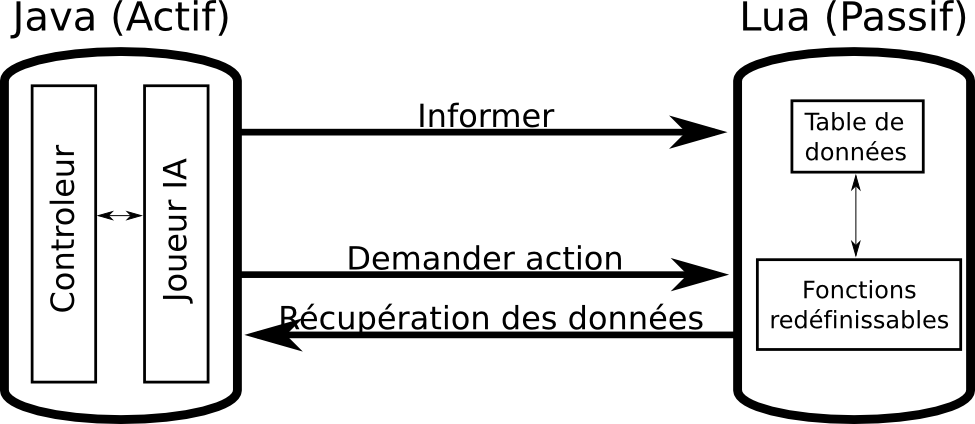
\includegraphics[scale=0.3]{Images/javalua.png}
			\end{center}
			\nopagebreak
			Nous avon donc créé une table d'informations relative à la donne en cours, manipulés directement par le programme Java :\\
			\begin{itemize}

			\item tarot.main : une table qui représente la main du joueur en question;

			\item tarot.legal : une table indiquant l’ensemble des cartes légales à tout moment;

			\item tarot.pli : un table indiquant le pli en cours;

			\item tarot.contrats : une table contenant les contrats par chaque joueur
			
			\item tarot.preneur : la position du joueur preneur
		
			\item tarot.entame : la position du joueur ayant entamé le pli
			 
			\end{itemize}
			Ensuite une série de fonctions, dites “demander”, qui seront appelées par le programme Java, demandant une réponse de la part de l’IA:\\
			\begin{itemize}
			    \item tarot.demander.contrat : doit renvoyer l’entier représentant le contrat souhaité
			    \item tarot.demander.ecart : doit renvoyer une table de 6 cartes
			    \item tarot.demander.carte : doit renvoyer une carte légale à jouer
			\end{itemize}
			Ecrire une intelligence artificielle dans ce contexte consiste à redéfinir les trois fonctions “demander” afin de créer le comportement souhaité.\\

			Lorsque un joueur IA est créé, il exécute un script par défaut qui initialise ces objets, et définit un comportement par défaut. Ensuite, un peut passer un nouveau script qui 				contient une définition des fonctions “demander” qui remplacera la version par défaut. Ainsi il n’est pas nécessaire d’écrire une IA complète pour définir un comportement simple.


\subsection{Les stratégies du joueur par défaut:}

Le tarot est un jeu relativement complexe, et les stratégies utilisées relèvent plus de l’instinct du joueur, d’estimation de probabilités, et d’expérience que de calcul. Nous avons donc pris la décision d'implémenter un comportement de jeu semblable aux conseils donnés à nouveau joueur.\\
Notre IA utilisera donc des stratégies relativement simples et peu risquées, mais aura l’avantage de savoir mieux compter les cartes jouées. On espère ainsi créer une IA qui jouera correctement.\\

Il y a trois composantes à la stratégie d’un jeu de tarot, la prise de contrat, la constitution de l’écart, et le jeu de la carte. Chacun de ces composantes présente un défi différent.\\

La prise de contrat consiste à estimer la “force” de sa main. La force d’une main est une notion plus complexe que la simple somme des cartes fortes, mais dépend aussi de particularités comme le nombre de cartes à chaque couleur, la probabilité que les cartes fortes de la main soient réellement utiles, et la probabilité de “voler” des cartes à l’adversaire.\\

Notre IA évalue sa main en affectant une valeur à certaines cartes, et à certaines configurations qui s’avèrent souvent utiles lorsqu’on est le joueur preneur.\\
Ainsi, le 1 d’atout, (dit “le petit”) un “bout” qui permet de réduire la difficulté de son contrat, est une carte prenable par l’adversaire, on affecte donc une valeur plus grande à cette carte si elle est accompagnée d’un grand nombre d’atouts qui permettent d’éviter de devoir jouer le petit à un moment inopportun.\\
La présence de “coupes” (aucune carte à une couleur donnée) ou de “singlettes” (une seule carte à une couleur donnée) est aussi pris en compte, puisqu’elles permettent de voler des points adverses lorsqu’on pourra jouer des atouts à ces couleurs.\\

Ces paramètres sont pris en compte et on définit des seuils qui correspondent à différents contrats. Lorsqu’un seuil est dépassé, notre IA demandera à jouer le contrat en question s’il est disponible.\\


Lors des contrats “petite” et “garde” les cartes du “chien” sont révélés et ajoutés à la main du preneur, qui doit ensuite constituer un “écart” comportant autant de cartes. Cet écart est posé dans les plis du preneur et compte pour son total de points en fin de partie.\\

Le preneur profite de la phase de constitution d’écart pour “améliorer” sa main en créant des “coupes” et “singlettes”, et le joueur peut aussi poser certains points (les Rois sont interdits à l’écart, mais les autres têtes peuvent y être) afin de ne pas les perdre lors du jeu de la carte.\\

Notre IA identifie donc les couleurs où il peut écarter assez de cartes pour créer des coupes, et s’il ne peut pas il cherche ses cartes à points et les met à l’écart.\\


Lors de la phase de jeu de la cartes un comportement de base est développé, ainsi qu’une collection de comportements spéciaux qui sont appliqués si certaines conditions sont remplies.\\

Le comportement de base consiste en estimer la probabilité (un calcul de probabilité pondéré par le fait que le preneur possède généralement une bonne main) qu’une carte valable soit remportée par son équipe, la jouer si le risque est assez bas, sinon tenter de jouer une carte sans valeur.\\
Lorsque le joueur IA doit entamer un pli, il cherche à jouer une couleur qui a déjà été jouée, préférablement une couleur où il a beaucoup de cartes et où il ne possède pas de cartes qu’il pourrait perdre.\\

Ensuite des comportements spéciaux sont ajoutées:\\
L’ouverture: Un joueur IA placé juste avant le preneur joue une carte sans valeur à une couleur qui n’a pas été jouée, permettant ainsi d’identifier les coupes du preneur et permettre à ses équipiers de jouer leurs cartes valables si le preneur ne coupe pas.\\

L’excuse: La carte de l’excuse est un cas particulier. Il peut être joué à tout moment, ne permet pas de remporter le pli, et revient au camp qui l’a joué, sauf si il est joué au dernier pli où il est donné au camp adverse.\\
L’IA affecte une priorité à ses cartes en fonction de leur valeur dans le jeu (le petit et les têtes) et jouera l’excuse pour éviter de jouer une de ces cartes si il risque de la perdre, et tentera de se débarrasser de l’excuse lors d’un pli qu’il ne peut affecter lorsqu’il n’aura plus de cartes à protéger. En dernier recours il jouera l’excuse à l’avant dernier pli afin d’éviter de le donner à l’adversaire.\\

Au total 7 comportements spéciaux sont programmés, fournissant à l’IA assez de subtilité pour permettre un jeu intéressant et éviter d’avoir une IA “frustrante” qui joue des cartes causant l'échec de son équipe.\\

	\section{Interface graphique}
		Le plugin Android disponible dans Eclipse permet de simplifier la création d'interface graphique.
		Chaque interface graphique est décrite dans un fichier xml, mais peut être représentée de manière
		visuelle à partir d'une fenêtre où des éléments peuvent être ajoutés par glisser/déposer.\\
		Une interface graphique définie en XML sera aussi générée comme une ressource dans la classe statique
		R. Le nom du fichier xml, par example accueil.xml permet de retrouver le layout dans le code java au
		travers de R.layout.accueil.\\
		Une Interface Utilisateur Android est composée d’une hiérarchie d’objets appelés Views (Vues).
		Une View est un objet à dessiner, utilisé comme un élément de l’interface utilisateur. Cela peut être un bouton, une image ou tout simplement du texte comme dans notre cas. Chacun de 			ces objets est une sous-classe de la classe View. Et la sous-classe qui prend en charge le texte est TextView.\\
		
		\subsection{Application native Android ou application Web ?}
			Notre encadrant Matthieu Lafourcade nous a un jour conseillé de programmer notre jeu de tarot sous la forme d’une application Web, plutôt qu’une application Android. Les 				avantages de cette approche sont multiples :\\
			\begin{itemize}
			    \item Compatibilité avec les différents systèmes, du moment que le navigateur web respecte et supporte les standards du Web (définis par le W3C).
			    \item Pas de mises à jour à télécharger
			    \item Utilisation de technologies mieux connues (JavaScript, HTML, CSS)
			\end{itemize}

			Cependant, elle a aussi ses inconvénients, parmi lesquels le fait qu’elle doit être chargée à chaque utilisation, alors qu’une application native est accédée depuis la mémoire 			du téléphone. À cela s’ajoute le fait que nous avions envie de faire ce projet entre autres pour découvrir les multiples aspects de la programmation Android. L’avantage d’une 				application Android sur une application Web est en particulier son intégration avec le système : on y accède directement, sans passer par un navigateur ; on a un menu (bouton 				Menu du téléphone) pour l’application, un système de préférences en cohérence avec les autres applications. De manière plus générale, on a accès à toutes les possibilités du 				système Android, là où une application Web n’aurait accès qu’à une partie de ces fonctionnalités. Choisir de développer une application Android est donc un moyen de proposer une 				expérience utilisateur la plus agréable, ergonomique et cohérente possible.\\
		\subsection{Structure de l’application}
			Une application Android se compose d’unités appelées « activités ». Notre application est ainsi composée de quatre activités :\\
			\begin{itemize}
			    \item Splash screen
			    \item Menu principal
			    \item Écran de préférences
			    \item Écran de jeu
			\end{itemize}

			Le splash screen contient une simple image d’accueil, et disparaît au bout de quelques secondes ou à un toucher de l’écran, pour laisser place au menu principal. Celui-ci est 				une interface simple comprenant plusieurs boutons : Commencer une partie, Reprendre une partie [seulement si partie en cours/enregistrée ?], Options. Dans cette activité, le 				bouton Menu du téléphone permet d’afficher un menu comprenant uniquement un bouton vers les préférences. De fait, cette fonctionnalité est inutile car redondante avec le bouton 				Options dans l’activité, mais nous avions envie d’essayer cette possibilité du SDK Android. [bof… de toute façon il faudrait peut-être décider, soit de virer le menu, soit de 				virer le bouton Options dans l’écran d’accueil ? ][ou de laisser les deux suivant l’habitude des utilisateurs (je cherche souvent un bouton options dans les applications et 				c’est souvent grâce au bouton menu qu’on y accède) possibilité d’argumentation de ce point en disant qu’il ya les deux pour les différents types d’utilisateurs]\\


		\subsection{Gestion des préférences}
			Afin de mettre en application les principales variantes du tarot, il était primordial dans ce projet de coder une partie où l’on peut choisir sa propre variante du jeu.\\
\begin{center}
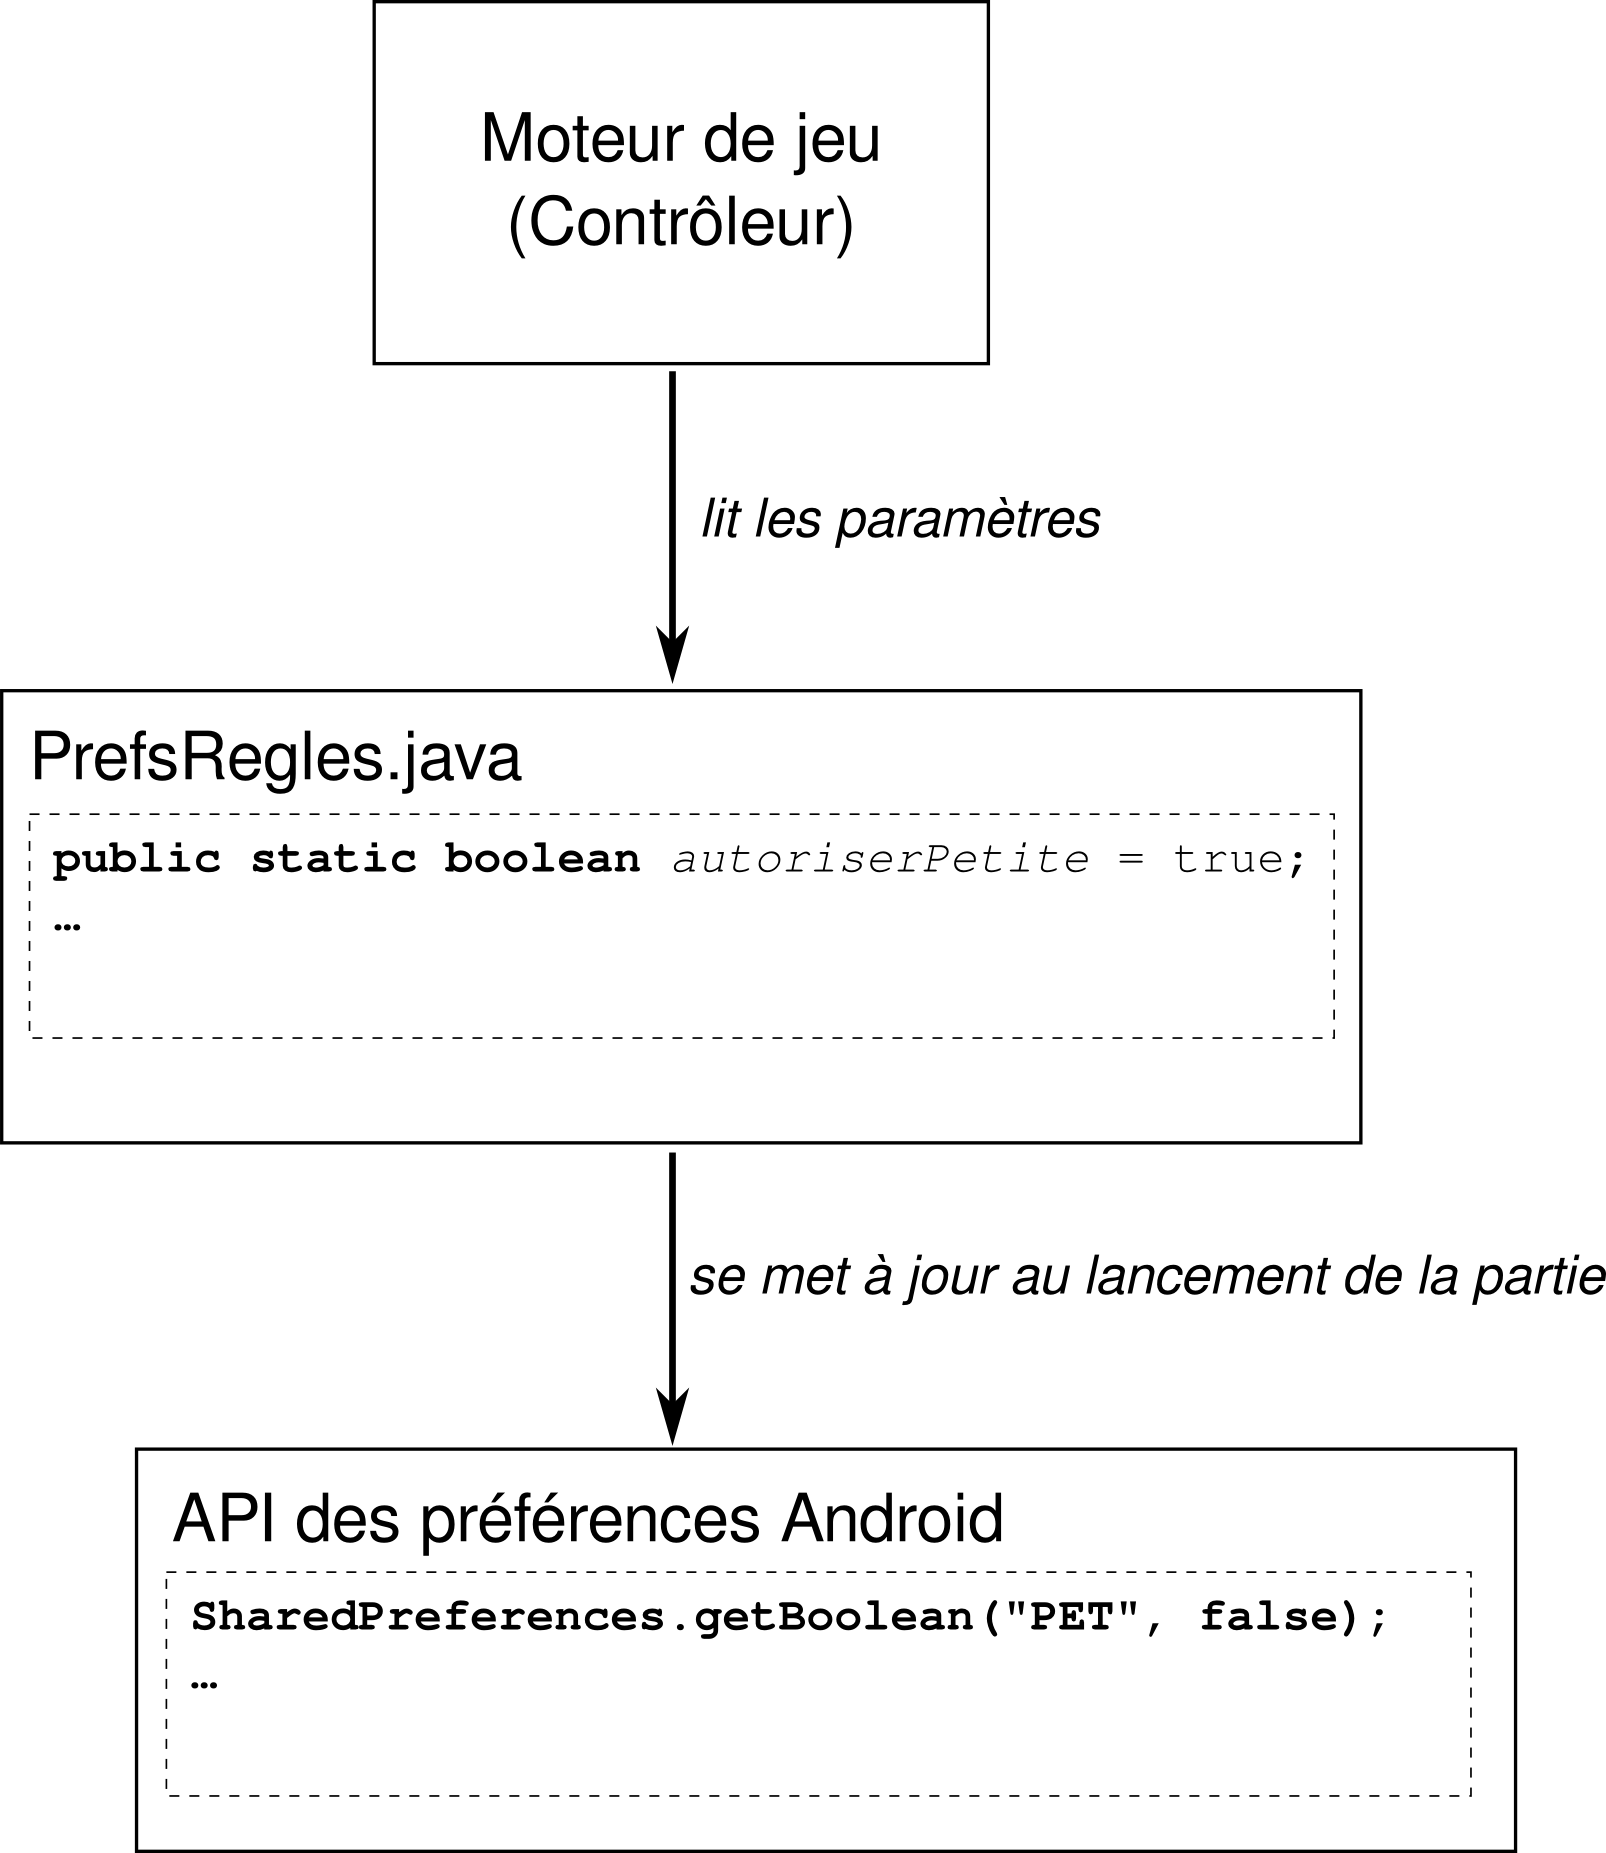
\includegraphics[scale=0.3]{Images/prefs.png}\\
\end{center}
]

D’apres le schéma, on peut voir de quelle manière les préférences ont été gérées. On a créé une classe nommée PrefsRegles contenant toutes les préférences et permettant de les mémoriser, qui est indépendante du moteur de jeu. Ce dernier au moment où on lance une partie lit ainsi les paramètres de cette classe. En faisant appel aux fonctions de l’API (ici getBoolean) qui consiste à récupérer les valeurs des préférences, et donc mettre à jour les paramètres de la classe PrefsRegles.


		\subsection{L’activité principale : l’écran de jeu}
			Au chargement de l’activité principale, l’écran de jeu, une nouvelle instance de la classe Partie est créée. Ensuite sont instanciés un « 				JoueurGraphique », correspondant à l’utilisateur de l’appareil/du téléphone, et trois « JoueurIA » (pour une partie à quatre joueurs), correspondant aux intelligences 				artificielles. On insère enfin ces joueurs dans la Partie, avec la méthode setJoueur. La partie peut démarrer.\\
			La classe Partie hérite de la classe Thread, ce qui lui permet d’être exécutée de manière concurrente et non bloquante en même temps que le thread principal de 			l’interface utilisateur. Ceci était indispensable pour que l’utilisateur ait toujours le contrôle sur son téléphone, quel que soit la situation. Sans cela, il serait par exemple 				complètement bloqué en attendant que les IA jouent leur carte ou fassent leurs annonces. Pour lancer la partie comme thread, on utilise la méthode start(), qui va appeler la 				méthode run(), que nous avons redéfinie pour lui faire exécuter lancerPartie().\\
			Quand le moteur de jeu exécute une demande de carte sur le JoueurGraphique, celui-ci va passer en mode « choix de carte » et lancer une boucle vide qui s’arrêtera quand le 				joueur aura choisi une carte. Pour le moteur de jeu, le temps s’arrête entre l’appel de demanderCarte(), par exemple, et le retour de cette méthode.\\

	\section{Réseau}

		Un de nos objectifs secondaires était la possibilité de jouer en ligne. Cependant, plusieurs problèmes nous ont bloqués dans cette tâche.
		En premier lieu, dans l’optique d’une architecture client-serveur, comme le moteur de jeu du serveur est le même que celui dans un client qui joue en local, le problème se posait 			d’éviter la duplication de code. Comment avoir une partie commune entre deux programmes, l’application Android (client) et le serveur, sans avoir à effectuer des allers-retours 			fastidieux à chaque modification du code ? De plus, notre objectif ultime était que, au même titre qu’un serveur installé sur un ordinateur fixe, n’importe quel terminal Android puisse 			héberger une partie multijoueur. \\
		\\ 
		Le second problème que nous avons rencontré quand nous avons travaillé sur cet aspect, était le manque de documentation concernant la programmation réseau sous Android. L’ensemble de 			l’API Android étant déjà assez difficile à prendre en main, et pas toujours suffisamment documenté, il nous était ainsi très difficile de comprendre le fonctionnement de l’aspect 			réseau, pas du tout documenté et encore plus obscur pour nous, d’autant plus que l’on manquait aussi d’expérience dans la programmation réseau en général.\\
		\\ 
		Ces problèmes nous empêchaient d’avancer, et le temps venait à manquer. La partie réseau a donc été abandonnée pour pouvoir mieux terminer les autres parties et les améliorer. On peut toutefois 			noter quelques points importants.\\
		\\ 
		Premièrement on peut noter que nos structures de données ont été construites de façon à pouvoir rajouter chaque méthode de communication à la structure sans la changer.\\
		Effectivement nous avons créé une classe croupier dont le seule rôle est la communication entre notre moteur de jeu et les joueurs, il suffirait donc de faire des changements au croupier 			si on voulait par exemple rendre possible un jeu en réseau, ou même une partie grâce à un réseau Bluetooth, sans avoir à toucher au moteur et au déroulement du jeu.\\
		\\ 
		Certaines structures pour une partie en réseau ont été commencées. L'idée était qu'un joueur puisse lancer une partie en ligne et que la partie commence aussitôt que le nombre de joueurs 		requis se soit connectés. Pour cela si un joueur lance une partie réseau, un serveur est lancé qui accepte les connections et crée un thread pour chaque joueur connecté. La 			communication se fait suivant un protocole et en envoyant des objets serializés. Les seuls objets nécesaires pour cette communication sont: une carte, un vecteur de carte, et 		finalement un objet contenant un entier qui représente une requette précise du protocole et un string pouvant contenir un message supplémentaire.\\
		\\ 
		Du côté du joueur, une fois la connection établie, tout ce passe de la même façon que le jeu hors ligne.\\













\chapter{L’interface Homme-Machine}
	Le jeu du Tarot est un jeu de cartes à 4. Il se joue principalement autour d’une table. Chaque joueur a 18 cartes dans sa main (et jusqu’à 24 cartes pour un jeu à 3).\\
	Le format des cartes est plus long que celui du poker, par exemple. Celà vient du fait qu’il serait plus difficile de jouer avec ces cartes lorsque le nombre de cartes distribuées est assez 		grand. Les dimensions classiques d'une carte de tarot sont de 61 * 112 mm. \\
	\\  
	Développer une application de jeu de Tarot sous Android implique forcément de s’inspirer de la réalité. Cependant, le gameplay ne pourra être le même. La question est donc : comment représenter 		la réalité de telle manière à ne pas perturber le joueur sur un smartphone ? Ajuster les cartes sur un si petit écran peut très vite devenir difficile.\\

	\section{Rendre son application compatible avec toutes les tailles d’écrans}
	
		Les développeurs Android ont peu de chances. Le nombre de téléphones aux caractéristiques totalement différentes augmente chaque mois. Et cibler un seul modèle n’est pas gagnant.\\
		Google publie donc des statistiques concernant les écrans utilisés :\\
		\begin{center}
			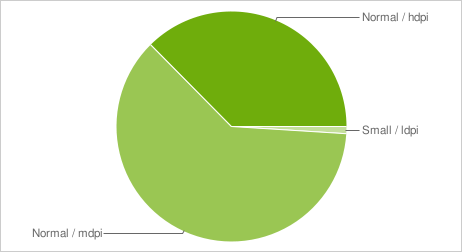
\includegraphics[scale=0.9]{Images/stats-screens-density.png}
		\end{center}
		Les écrans hdpi (3.3”-4”) et mdpi (3”) sont les plus courants. Bien sur, c’est légèrement plus complexe que ça. J’ai omis de parler de la densité. Android répartit les différentes 			tailles et densités ainsi :
		\begin{center}
			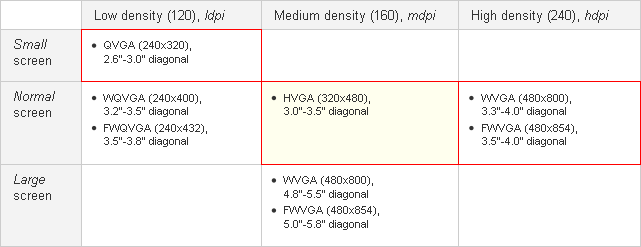
\includegraphics[scale=0.7]{Images/resolution-android.png}
		\end{center}
		L’écran et la densité par défaut sont en rouge.\\

		Supposons par exemple, que l’on souhaite utiliser un fichier PNG de 24 x 24 pixels, et que l’application s’exécute sur un écran de taille normale mais avec un résolution WVGA (haute 			résolution). Android modifiera alors la taille du fichier PNG pour qu’il fasse 36 x 36 pixels. Ce traitement est automatique, certe, mais les images sont moins nettes.\\

		Pour gérer cette multitude d'écrans, Android se base sur la configuration de son fichi erAndroidManifest.xml mais également sur le nom des répertoires de ressources (répertoire res/). 		Il est possible de leur rajouter des qualificatifs :\\
		\begin{itemize}
   			\item pour les différentes taille des écrans : -large, -normal, et -small

   		 	\item pour les différentes densités : -hdpi, -mdpi, et -ldpi

		\end{itemize}

	\section{Afficher le jeu à l’écran}


		Imaginons que le problème de taille et de densité soit réglé. Désormais il faudrait afficher le jeu tel que l’on peut le voir en réalité dans sa main.
		\begin{center}
			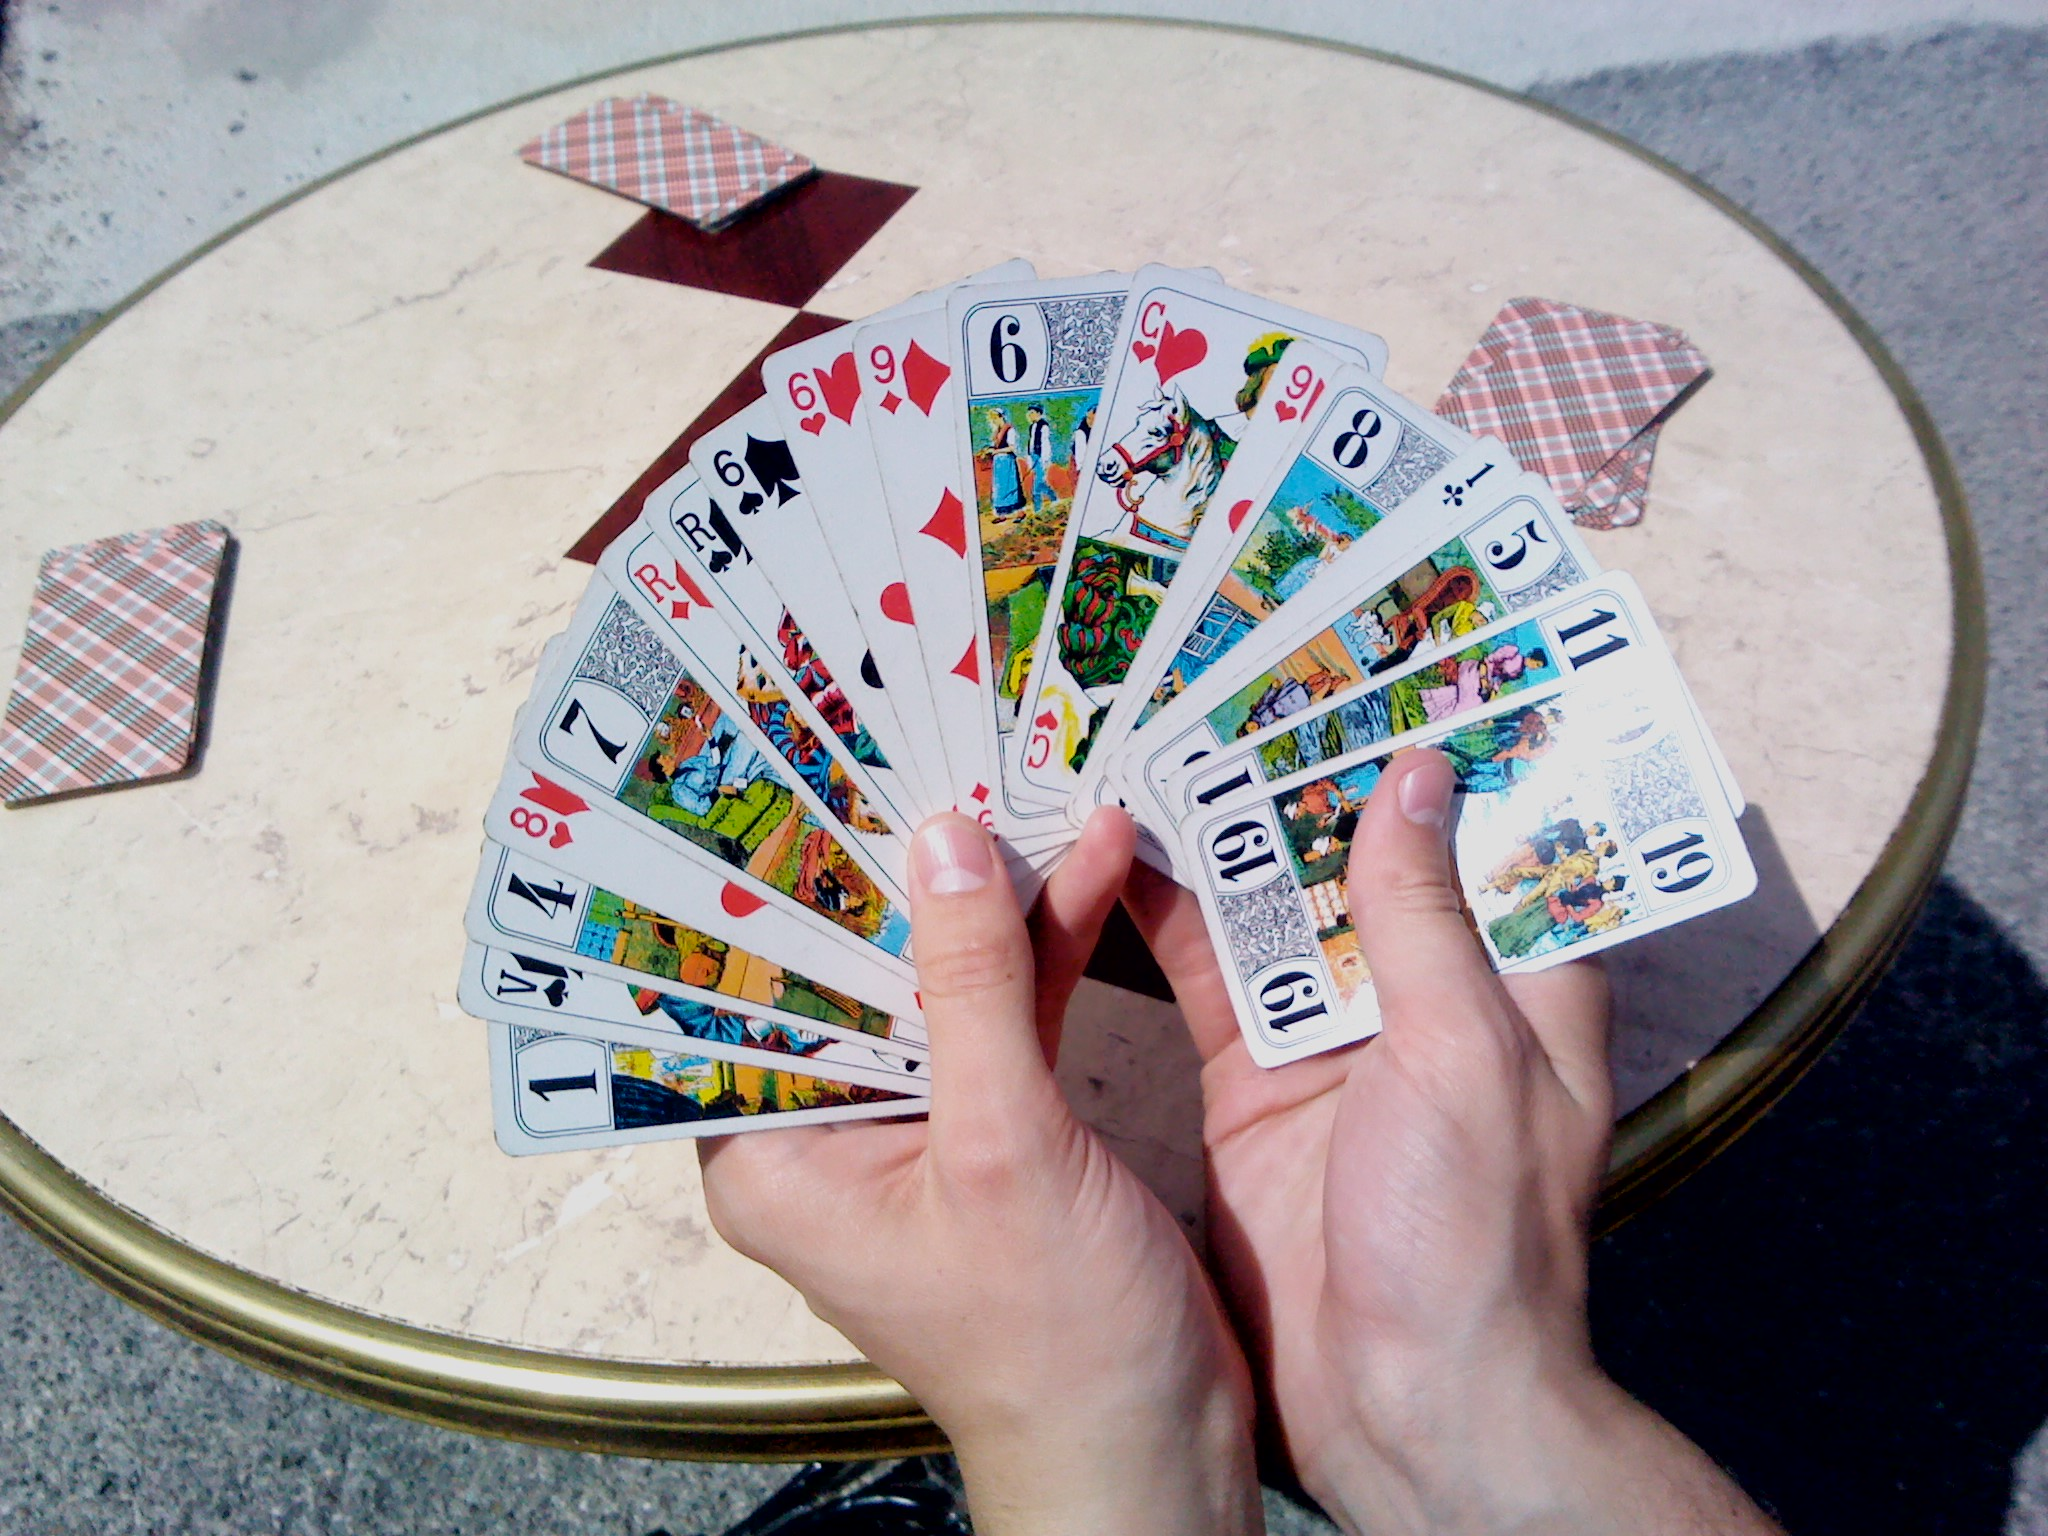
\includegraphics[scale=0.15]{Images/1.jpg}
		\end{center}

		On se rend très vite compte, qu’il n’est pas possible d’afficher les cartes complètes. Même dans sa main, on ne peut se permettre de les tenir de manière à ce qu’elles soient 			entièrement visibles. Reprenons ce système sur notre application. 

		\begin{center}
			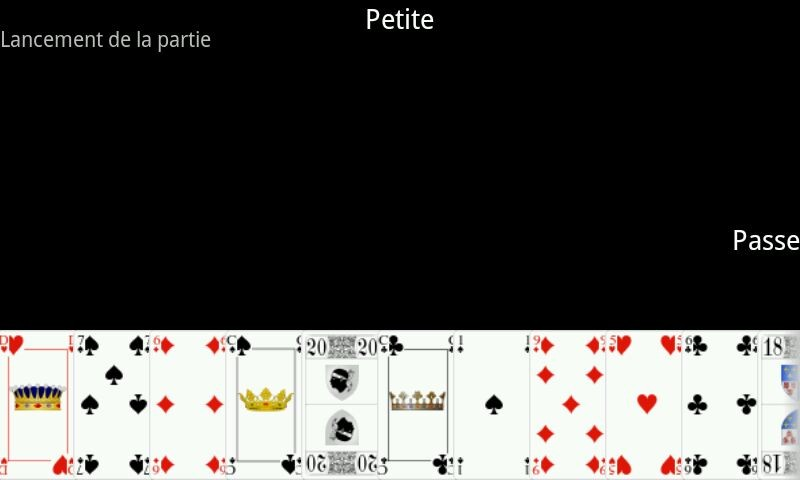
\includegraphics[scale=0.6]{Images/main.jpg}
		\end{center}
		Les cartes ne sont pas affichées dans leur totalité. Mais on ne les coupe pas sur leur hauteur. Celà permet de bien voir quelques cartes avont nous en main.\\
		Cependant, il n’est pas possible d’afficher toutes les cartes sur l’écran. Ce problème est résolu par un scroll qui permet très facilement de faire défiler les cartes de notre main.
		On pourrait rapporter celà au fait qu’après distribution des cartes, on les regarde les unes après les autres.\\
		Ensuite, on viendrait à se demander pourquoi ne pas les afficher sur l’écran comme en réalité, c’est à dire en éventail. Pour diverses raisons, nous n’avons pu faire ce choix.\\ 		Premièrement, java et xml ne permettent à eux seuls des affichages de cartes aussi complexes. Deuxièmement, celà prendrait beaucoup trop de place sur l’écran.\\

		Ensuite, que voyons nous lorsque l’on joue entre amis ? Le dos des cartes de chacun, ainsi que le nombre qu’il a en main. Nous avons donc décider d’afficher sur le cotés et en haut de 		l’écran, les mains des 3 autres joueurs.\\
		Pendant la partie, les cartes sont posées sur table. C’est pareil pour l’application. Les cartes jouées s’affichent au fur et à mesure au centre de l’écran.
		
	
	\section{Simuler la réalité}
		Que peut il se passer pendant le jeu ? Doit-on simuler le fait de faire tomber ses cartes ? Accepter la tricherie comment celà pourrait arriver dans la réalité ? Simuler la distribution 			des cartes ?\\

		Avant le jeu :\\
   		Le Tarot se joue à 4 joueurs (3 ou 5 pour des variantes). Il est facile de représenter à l’écran le fait que 4 joueurs sont présents. Cependant il est impossible de voir les autres 			joueurs sur cet écran. Surtout quand ces joueurs sont des IA.\\
   		Le preneur joue contre les 3 autres joueurs qui représentent la défense. La seule façon de le montrer sur l’application, est de désigner le preneur.\\
    		Les cartes ne doivent jamais être mélangées (sauf si elles ont été classées). C’est ce qui se passe pour l’application.\\
   		Un talon de six cartes aussi appelé le chien est constitué.\\
		\\  
		Personne ne doit avoir connaissance des cartes composant le chien. Chaque joueur prend son jeu dans les mains en prenant soin de le cacher aux autres joueurs. A l’écran, il n’y a aucun 			moyen de connaître les mains des autres joueurs. Ceci est un choix personnel. Nous n’acceptons pas la tricherie.\\ 
		\\  
		Début du jeu :\\
   		Le joueur placé à la gauche du donneur parle en premier; soit il passe soit il prend puis la parole est au joueur placé à sa gauche, et ainsi de suite. Pour notre application, les 			joueurs sont situés ainsi :\\  
		\begin{center}
			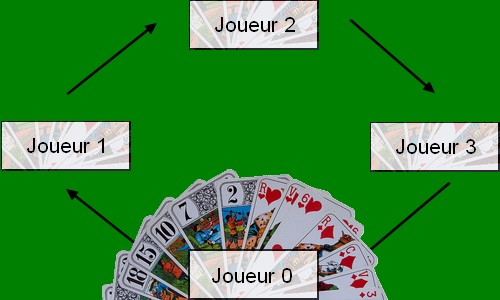
\includegraphics[scale=0.7]{Images/placement.jpg}
		\end{center}

		Si le joueur 0 distribue les cartes, alors le joueur 1 prendra la parole en premier. Et ainsi de suite.\\
   		Celui qui a fait la plus forte enchère dispose des cartes du chien ( sauf dans les cas de garde sans ou contre le chien ) qu'il doit montrer aux autres joueurs avant de le mêler à son 		jeu. Il écarte en suite six cartes de son jeu. Jusque là, c’est possible depuis notre application. Le fait que le chien appartiennent à la défense ou non, ne se voit pas mais se devine 			suivant le contrat du preneur. En réalité, le chien est rapproché du coté des défenseurs ou du preneur.\\
    		Le preneur s'engage à réaliser un minimum de points selon le nombre de bouts qu'il possède dans ses levées à la fin de la partie. Ceci est facilement représentable.\\
   		\\ 
		Déroulement du jeu :\\
  		Tous les joueurs partent avec le même nombre de cartes. Celui qui commence est celui placé à gauche du donneur. Chacun joue à son tour ( dans le sens des aiguilles d'une montre ) en 			mettant à chaque fois obligatoirement une carte sur la table, face visible. Ceci apparaît très bien sur l’application.\\
   		Les joueurs ne doivent pas sortir de carte avant leur tour de jeu, toute carte sortie est alors considérée comme jouée. Sur l’application, il n’est pas possible de joueur une carte en 		dehors de son tour.\\
    		Une carte non recouverte peut être reprise en jeu réel. Cependant, cette fonctionnalité n’a pas été implémentée dans notre jeu.\\


\chapter{Manuel d’utilisation}

Notre projet est deja disponible sur le Play Store (Andoid market).\\
Pour l'utiliser il suffit de :
\begin{itemize}
	\item ouvrir le Play Store
	\item télecharger notre application
	\item l'installation est automatique
	\item lancer l'application
\end{itemize}

Si on veut tester l'application sur un ordinateur il est possible d'utiliser l'émulateur. Cette procedure est mahlheureusement plus difficile et il peut avoir des differences entre l'emulateur et un portable.\\
Pour pouvoir lancer notre projet sur un émulateur il faut :
\begin{itemize}
	\item installer eclipse
	\item recuperer notre code source à partir du cd
	\item installer le plugin adt sur eclipse
	\item créer une machine virtuelle (de préference avec la version 2.2 mais les versions plus récentes devraient fonctioner aussi
	\item lancer le projet avec cet machine virtuelle
	\item lancer l'application dans l'émulateur \\
\end{itemize}

Une fois lancée on voit un écran de chargement et un écran d’acceuil contenant un menu nous permet de choisir entre “commencer une partie” ou “options”. Ces options sont aussi disponibles depuis la touche menu du smartphone.
Une fois que l’on a cliqué sur le bouton “commencer une partie”, un nouvel écran de jeu apparaît.\\
Les autres joueurs choisissent leurs contrats qui s’affichent au niveau de leur placement. Votre main est visible et vous pouvez donc choisir votre contrat, quand c’est votre tour, en cliquant sur le bouton “annoncer”.\\




		\begin{center}
			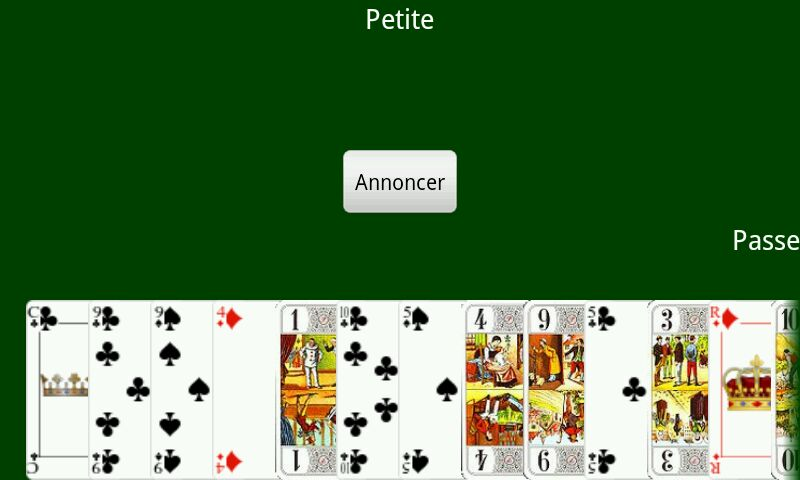
\includegraphics[scale=0.4]{Images/annonce.jpg}\\
		\end{center}
Pour annoncer, un menu déroulant s’ouvre, vous permettant ainsi de choisir le contrat. \\
		\begin{center}
			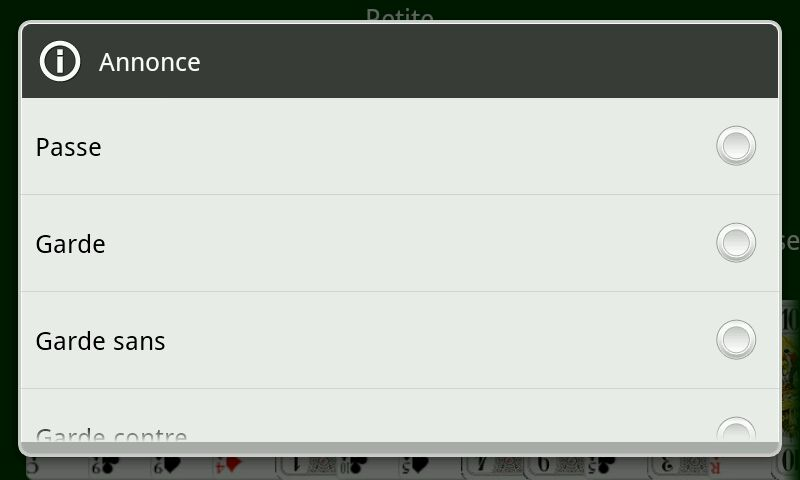
\includegraphics[scale=0.4]{Images/annonce2.jpg}\\
		\end{center}
Si vous passez, gardez sans ou contre, la partie commence. Sinon, si vous gardez, l’applciation vous demandera de faire votre écart. Il suffira de cliquer sur les cartes qui s’afficheront alors en vert. Vous pouvez recliquez sur une carte si vous ne souhaitez plus qu’elle fasse partie de votre écart. Si vous ne choisissez pas assez ou trop de cartes, la partie ne commecera pas. Quand votre écart est prêt, cliquez sur “Valider”.\\
		\begin{center}
			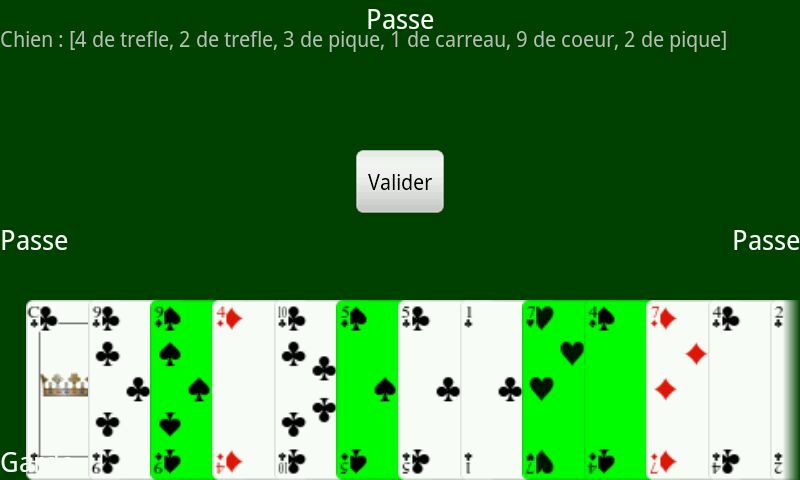
\includegraphics[scale=0.4]{Images/jeu.jpg}\\
		\end{center}
La donne peut enfin commencer. Chaque joueur peut poser une carte lors de son tour. La tricherie n’est pas possible. Seules les cartes légales sont cliquables. Pour sélectionner la carte à jouer, il suffit de cliquer sur cette carte dans votre main visible à l’écran.\\

		\begin{center}
			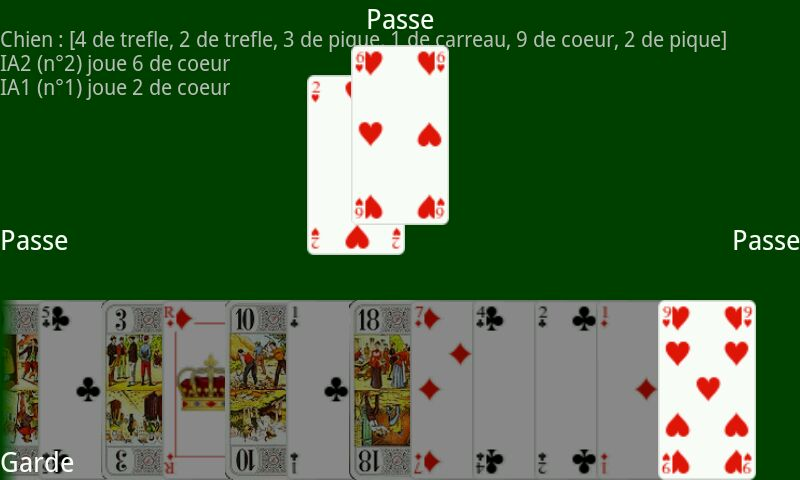
\includegraphics[scale=0.4]{Images/jeu2.jpg}\\
		\end{center}
Vous savez maintenant jouera notre jeu de tarot. Bonne chance.





\chapter{Perspectives et conclusions}
	\section{Perspectives}
		Ce projet a pour vocation d’être amélioré, et ce de multiples manières. En premier lieu, les objectifs de départ qui étaient définis comme « secondaires » pourraient être remplis.
		Cela inclut en particulier le jeu multijoueur en ligne, qui devrait permettre de jouer à plusieurs par Internet, ou même par WiFi ou Bluetooth, éventuellement avec des intelligences 			artificielles s’il n’y a pas assez de joueurs humains.
		L’intelligence artificielle devrait être perfectionnée et adaptée au jeu à 3 et 5 joueurs. Si à 3 joueurs le principe est fondamentalement le même – la stratégie est néanmoins 		légèrement différente du fait que les joueurs possèdent plus de cartes et peuvent plus facilement déduire les jeux des autres –, le jeu à 5 joueurs est en revanche fondamentalement 			différent. En effet, le preneur « appelle » un roi, et le joueur qui le possède sera son coéquipier en attaque. Tant que ce roi n’a pas été joué, les équipes d’attaque et de défense ne 			sont pas connues, ce qui complexifie grandement la stratégie. 
		Notre interface graphique, bien que tout à fait utilisable, pourrait être plus attrayante visuellement, et plus ergonomique. Les cartes s’afficheraient en éventail, on les ferait 			défiler et on pourrait faire un glissement du doigt vers le haut pour jouer une carte. Les cartes jouées pourraient être disposées de manière aléatoire et ainsi mieux refléter la 			réalité – il serait en revanche plus difficile de discerner qui a joué quelle carte.
		Notre interface graphique devrait aussi permettre de jouer à 3 ou 5 joueurs, ce qui n’est pas le cas actuellement.
			
	\section{Conclusions}	
		\subsection{Difficultés rencontrés}

Nombreux furent les obstacles rencontrés durant ce projet. En effet, les principaux objectifs à atteindre ne pouvant pas être atteints sans passer par une grande connaissance et de l’entrainement au niveau programmation, les passages qui nous ont pris du temps à effectuer ont étés de plusieurs sortes :

			\subsubsection{Difficulté de la programmation sous Android}
Android étant un système d’exploitation récent, le nombre de documents bien détaillés sur le fonctionnement d’une application sous Android et de sa programmation sont limitées. De plus, il est important de souligner que la programmation sous android est très riche et complexe et également difficile à assimiler.\\

			\subsubsection{Complexité du tarot}
Le déroulement d’une partie de tarot qui suit un avancement différent selon certaines conditions de départ, fait que cela ajoute une autre difficulté pour programmer le déroulement du jeu. De même qu’il y a également pas mal d’opérations à implémenter comme les scores.\\

			\subsubsection{Intelligence artificielle}
Dans un premier temps, l’intelligence artificielle à été un concept nouveau pour le groupe. Tout concept nouveau où l’on n’a pas les connaissances suffisantes pour avancer est un obstacle pour l’avancement du projet.\\
Dans un second temps, en suivant la complexité du tarot, des stratégies sont à adopter lorsque l’on joue au tarot régulièrement. Certaines stratégies ont donc dû être codées pour un bon fonctionnement du jeu.\\


		\subsection{Le fonctionnement de l'application}
			Malgrès les difficultées rencontrées nous sommes fière de ce que nous avons atteint.\\
			Notre moteur de jeu est très complet, comportants different variantes de jeu et un grand nombre de préferences. De plus le moteur de jeu implémente meme le jeu de tarot à 3, et le jeu de tarot à 5 joueurs qui comporte des differences importantes.
			La partie graphique nous sa posé beaucoup de problemes à cause des differentes tailles d'ecrans et les différences entre l'emulateur et les ecrans de portable mais nous avons tout de même reussi à créer une interface fonctionelle et intuitive.
			L'IA n'est pas encore parfaites mais elle sait faire un certain nombre de choses dont :
			\begin{itemize}
				\item faire un contract
				\item faire un écart
				\item a le niveau d'un joueur débutant 
	
			\end{itemize}
			Nous avons réussi à atteindre les objectifs du projet et ainsi obtenir une application de Tarot prête à être inclue sur le Play Store
			
	
		\subsection{Le travail en groupe }
		
			Le travail en groupe est quelque chose de difficile à géré il faut beaucoup de communication dans l’equipe.\\
			Les parties différentes d’un projet doivent être un maximum en contact pour ne pas s’éloigner les uns des autres.\\
			Si dans une équipe qui travalle sur un projet commun il n’y a pas de discution c’est rapidement le chaos. En effet il faut se mettre d’accord sur certains points. Notament en 				informatique car lorsque l’on doit relire le code d’une autre personne il faut pouvoir le relie le plus rapidement possible. Si un code n’est pas indenter ou indenter d’une 				façon bizarre ou pas tout le temps cela va être difficile à relire.\\
			Nous avons souvent du relire le code d’une autre personne pour corrigées certaines erreurs. C’est pourquoi nous avons décidé d’une convention d’indentation. Même si parfois il 			nous arrivé d’oublier d’indenter correctement en régle générale on a essayer de faire au mieux pour que notre code puisse être corrigé/débugger rapidement.\\
	


\chapter{Bibliographie}
\begin{itemize}
\item http://www.jeu-de-tarot.com 
\end{itemize}
\indent Page offrant une introduction au jeu de Tarot.\\
\begin{itemize}
\item http://www.fftarot.fr
\end{itemize}
\indent le site de la fédération française de Tarot.\\
\begin{itemize}
\item L'art du développement Andoid
\end{itemize}
\indent 3\ieme édition \\
\indent Pearson Education France\\
\indent ISBN : 948-2-7440-2495-5\\

\begin{itemize}
\item http://www.siteduzero.com/tutoriel-3-554364-developpez-des-applications-pour-android.html
\end{itemize}
\indent Tutoriel du site du zero

\begin{itemize}
\item "The evolution of Lua", R. Ierusalimschy, L. H. Figueiredo, W. Celes (2007)
\end{itemize}

\chapter{Annexe}
\begin{itemize}
\item Les regles de la féderation française den tarot
\item Diagramme de classes UML
\end{itemize}

\end{document}
